\documentclass[11pt]{amsart}
\usepackage{geometry}                % See geometry.pdf to learn the layout options. There are lots.
\geometry{letterpaper}                   % ... or a4paper or a5paper or ... 
%\geometry{landscape}                % Activate for for rotated page geometry
%\usepackage[parfill]{parskip}    % Activate to begin paragraphs with an empty line rather than an indent
\usepackage{graphicx}
\usepackage{amssymb}
\usepackage{epstopdf}
%\usepackage{subfigure}
\usepackage{caption}
\usepackage{subcaption}
\usepackage{amssymb}
\usepackage{amsmath}
\usepackage{amsthm}
\DeclareGraphicsRule{.tif}{png}{.png}{`convert #1 `dirname #1`/`basename #1 .tif`.png}
\newtheorem*{mydef}{Definition}
                                    % Activate to display a given date or no date

\begin{document}
\section{Unused Figures}




\begin{figure}
        \centering
        \begin{subfigure}{\textwidth}
                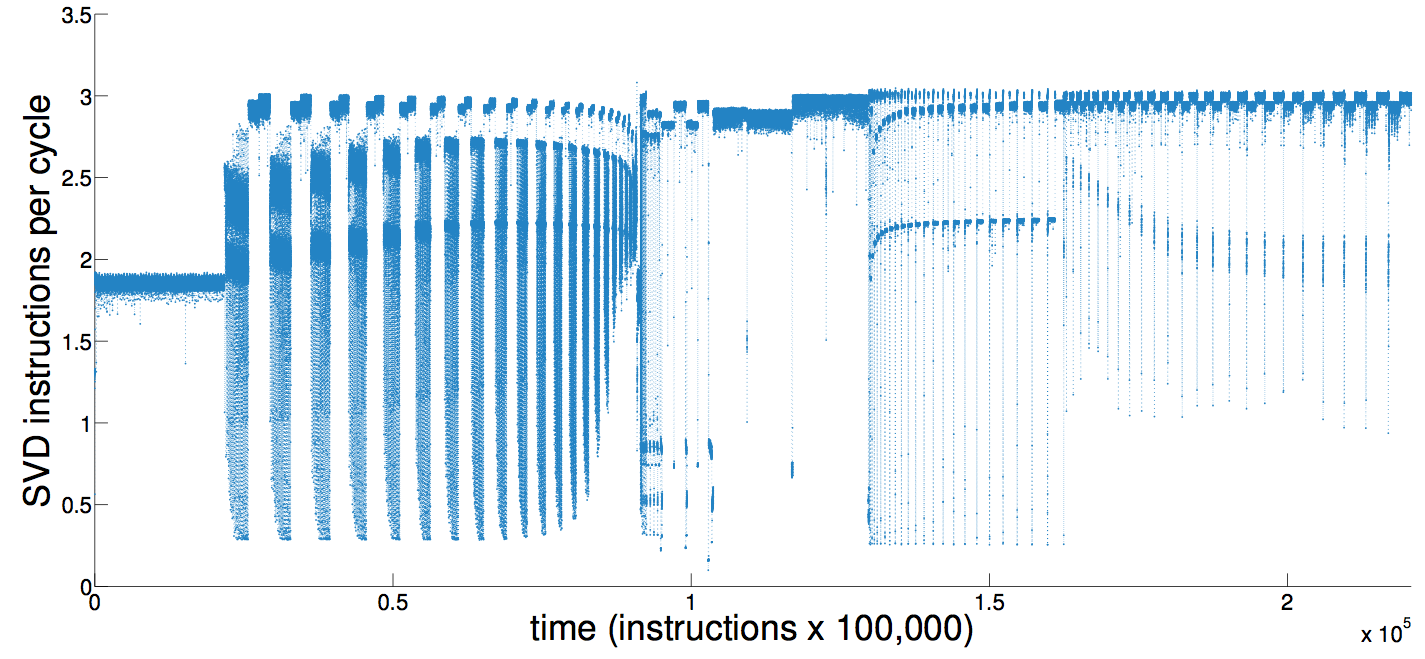
\includegraphics[width=\textwidth]{unused-figs/svdipcfull}
                \caption{SVD IPC without coloring}
                \label{fig:gull}
        \end{subfigure}%
        \newline
        ~ %add desired spacing between images, e. g. ~, \quad, \qquad etc.
          %(or a blank line to force the subfigure onto a new line)
        \begin{subfigure}[b]{\textwidth}
                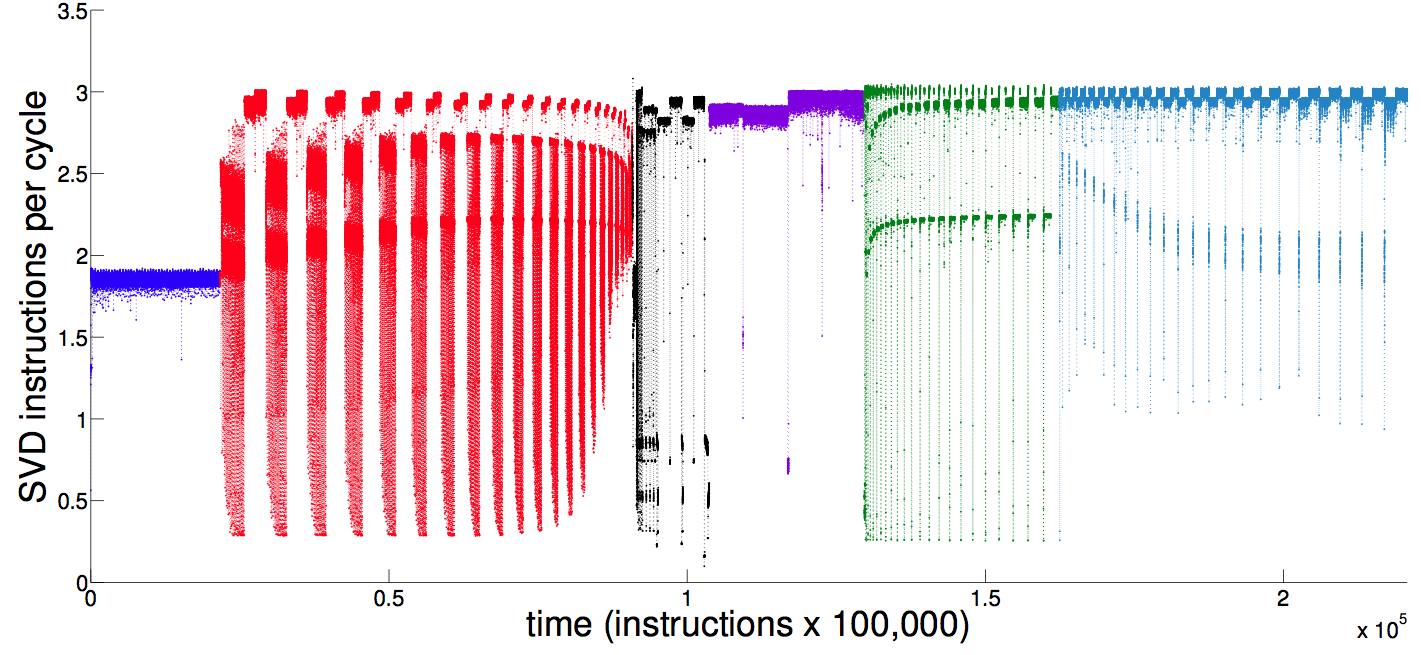
\includegraphics[width=\textwidth]{unused-figs/svdipcregimescolored}
                \caption{SVD IPC with coloring}
                \label{fig:svdFullColored}
        \end{subfigure}
        ~ %add desired spacing between images, e. g. ~, \quad, \qquad etc.
          %(or a blank line to force the subfigure onto a new line)
         \caption{SVD Full Time Series }\label{fig:svdFull}
\end{figure}





\begin{figure}
        \centering
        \begin{subfigure}{\textwidth}
                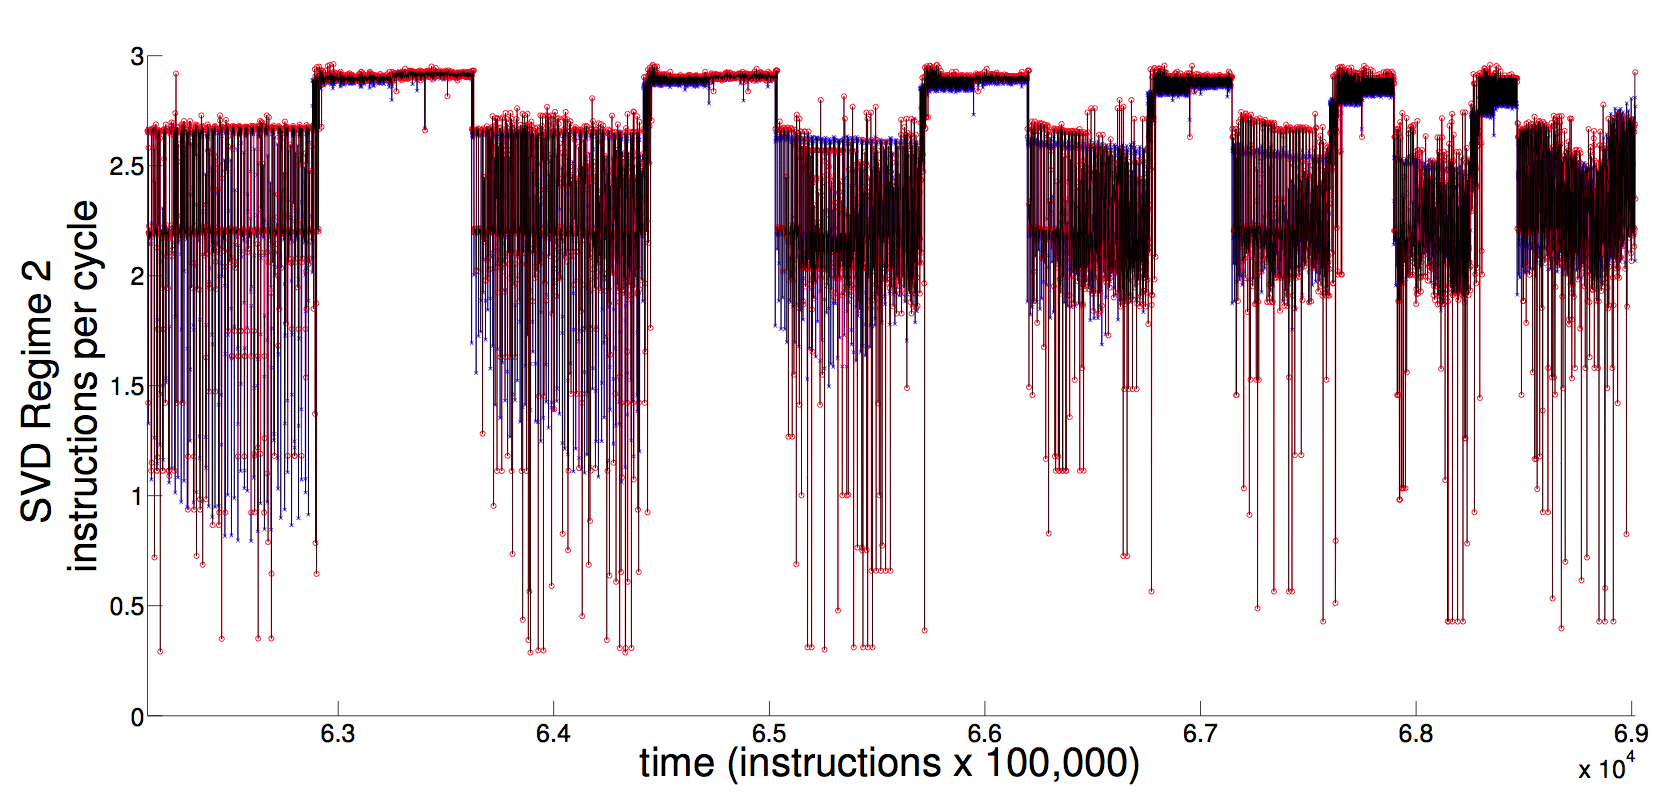
\includegraphics[width=\textwidth]{unused-figs/svdregime2prediction}
                \caption{SVD Regime 2 LMA Prediction}
                \label{fig:gull}
        \end{subfigure}%
        \newline
        ~ %add desired spacing between images, e. g. ~, \quad, \qquad etc.
          %(or a blank line to force the subfigure onto a new line)
        \begin{subfigure}[b]{\textwidth}
                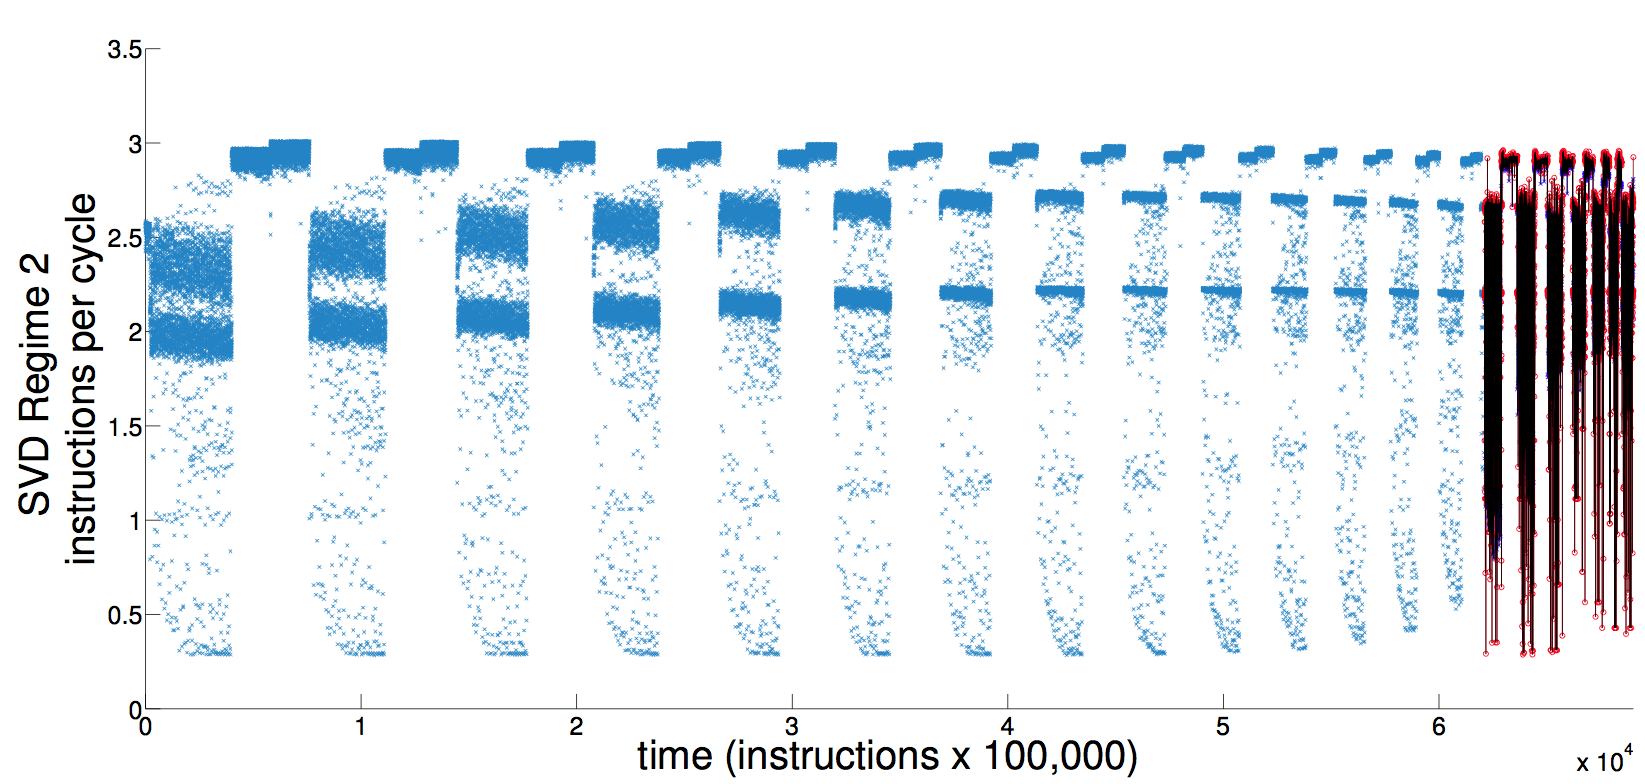
\includegraphics[width=\textwidth]{unused-figs/svdregime2predictionFULL}
                \caption{SVD Regime 2 LMA Prediction with Full Time Series}
                \label{fig:svdFullColored}
        \end{subfigure}
        ~ %add desired spacing between images, e. g. ~, \quad, \qquad etc.
          %(or a blank line to force the subfigure onto a new line)
         \caption{SVD Regime 2 LMA Prediction Figures }\label{fig:svdregime2prediciton}
\end{figure}






\begin{figure}
        \centering
        \begin{subfigure}{\textwidth}
                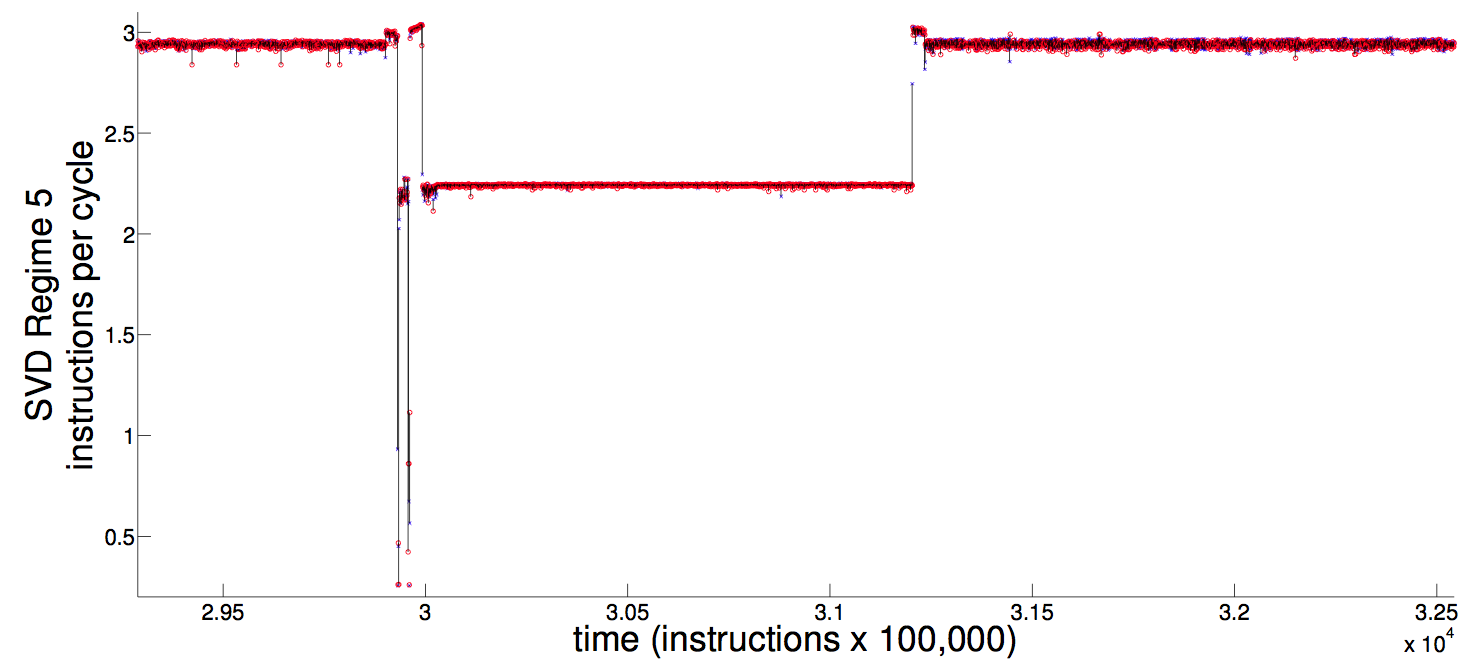
\includegraphics[width=\textwidth]{unused-figs/svdPrediction}
                \caption{SVD Regime 5 LMA Prediction}
                \label{fig:gull}
        \end{subfigure}%
        \newline
        ~ %add desired spacing between images, e. g. ~, \quad, \qquad etc.
          %(or a blank line to force the subfigure onto a new line)
        \begin{subfigure}[b]{\textwidth}
                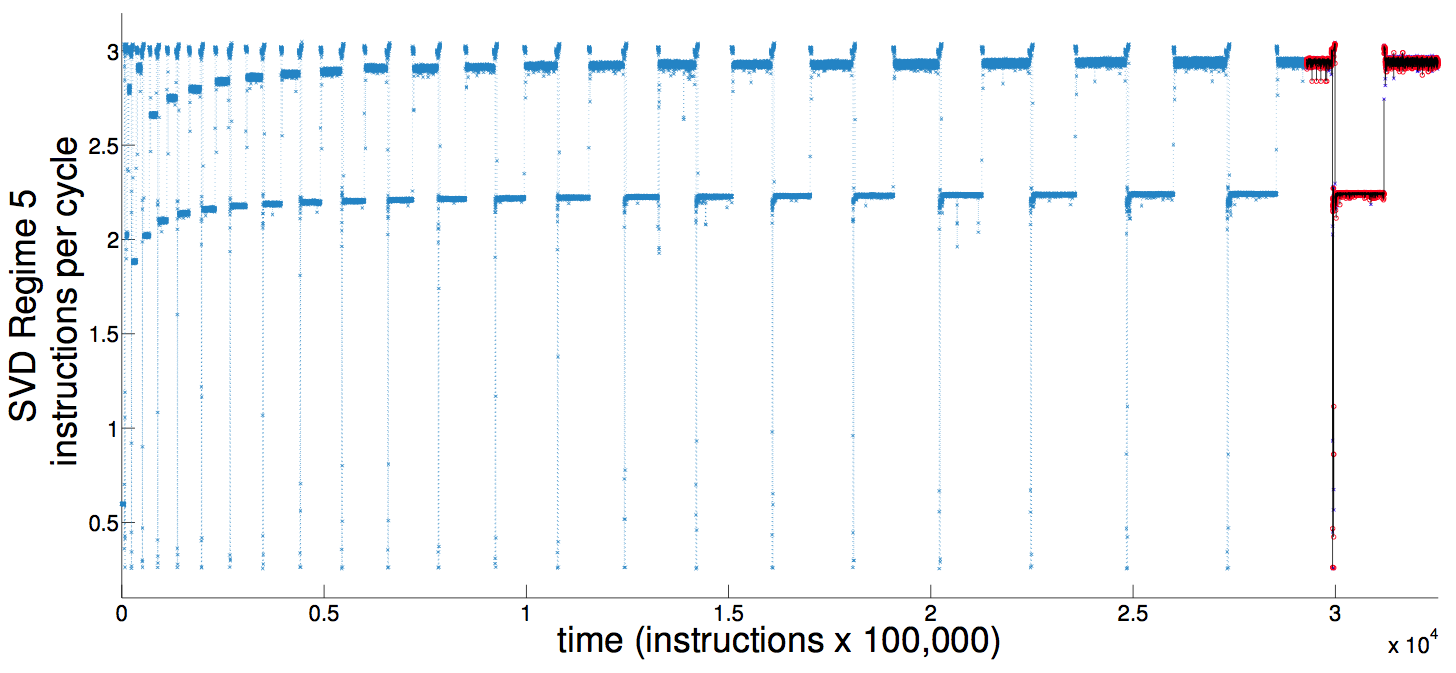
\includegraphics[width=\textwidth]{unused-figs/svdPredictionFull}
                \caption{SVD Regime 5 LMA Prediction with Full Time Series}
                \label{fig:svdFullColored}
        \end{subfigure}
        ~ %add desired spacing between images, e. g. ~, \quad, \qquad etc.
          %(or a blank line to force the subfigure onto a new line)
         \caption{SVD Regime 5 LMA Prediction Figures }\label{fig:svdregime5prediciton}
\end{figure}














\begin{figure}
        \centering
        \begin{subfigure}{\textwidth}
                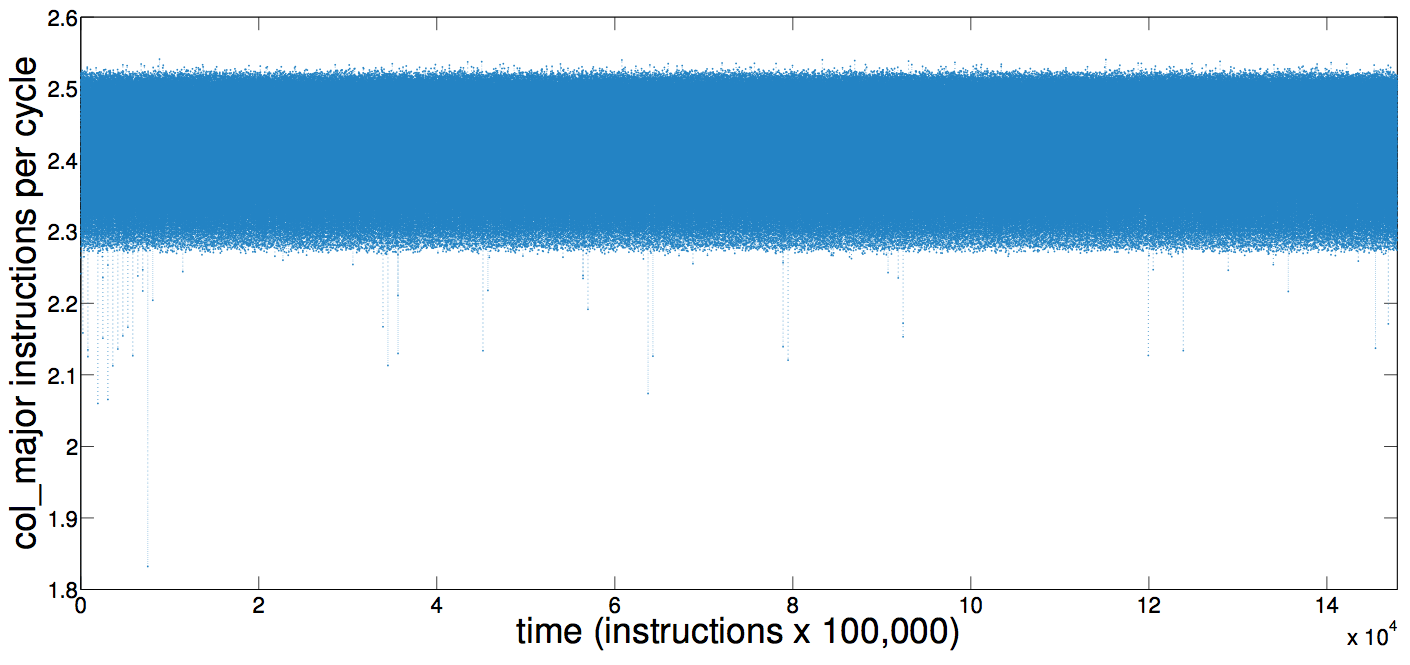
\includegraphics[width=\textwidth]{unused-figs/colfullts}
                \caption{col IPC  Full Time Series}
                \label{fig:gull}
        \end{subfigure}%
        \newline
        ~ %add desired spacing between images, e. g. ~, \quad, \qquad etc.
          %(or a blank line to force the subfigure onto a new line)
        \begin{subfigure}[b]{\textwidth}
                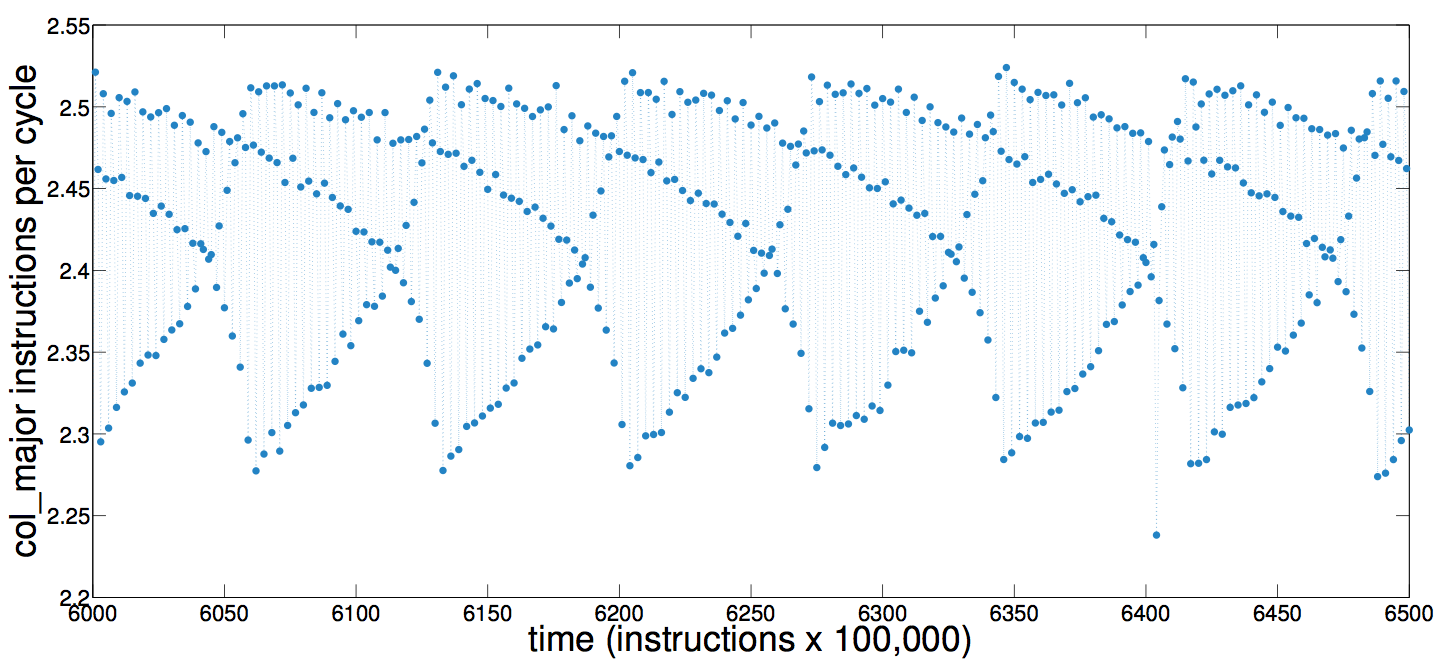
\includegraphics[width=\textwidth]{unused-figs/colshortts}
                \caption{col IPC  Short Time Series for structure illustration}
                \label{fig:svdFullColored}
        \end{subfigure}

        ~ %add desired spacing between images, e. g. ~, \quad, \qquad etc.
          %(or a blank line to force the subfigure onto a new line)
         \caption{col  Time Series }\label{fig:svdFull}
\end{figure}

\begin{figure}
        \centering
        \begin{subfigure}{\textwidth}
                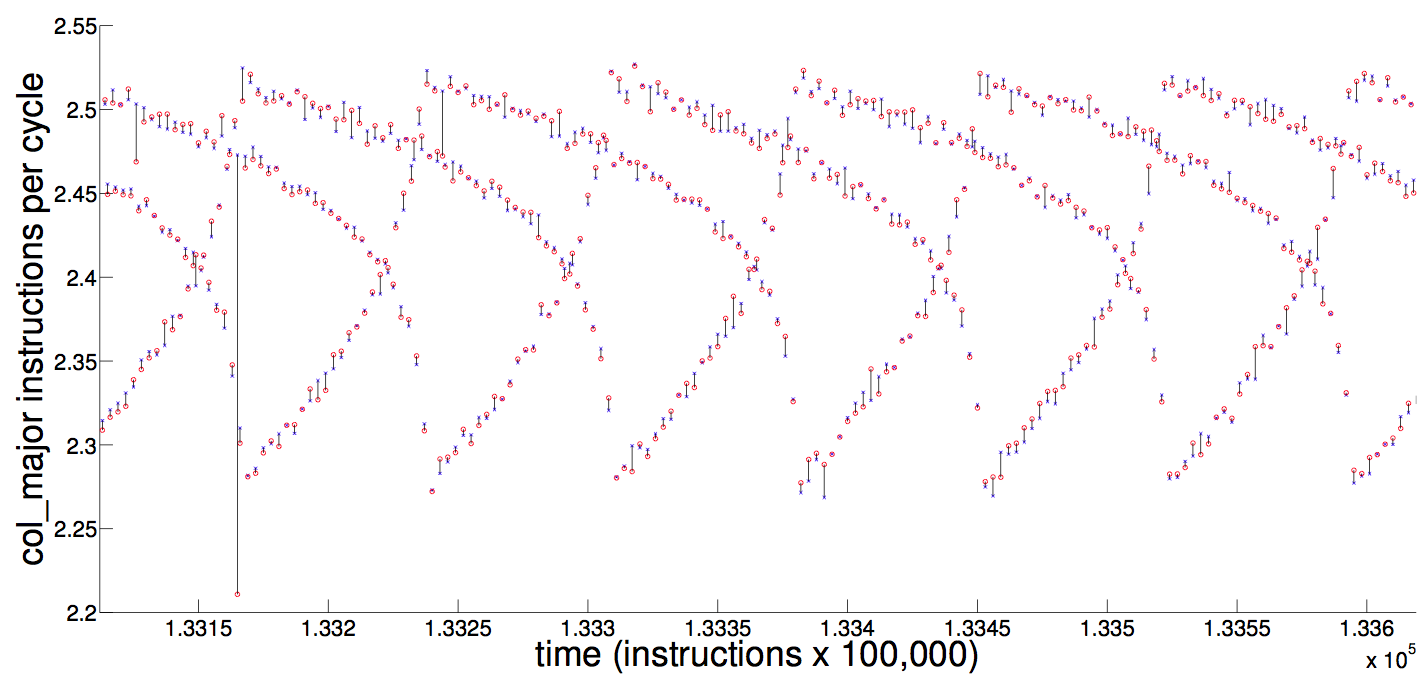
\includegraphics[width=\textwidth]{unused-figs/colPredShortTS}
                \caption{col IPC  Full Time Series}
                \label{fig:gull}
        \end{subfigure}%
        \newline
        ~ %add desired spacing between images, e. g. ~, \quad, \qquad etc.
          %(or a blank line to force the subfigure onto a new line)
        \begin{subfigure}[b]{\textwidth}
                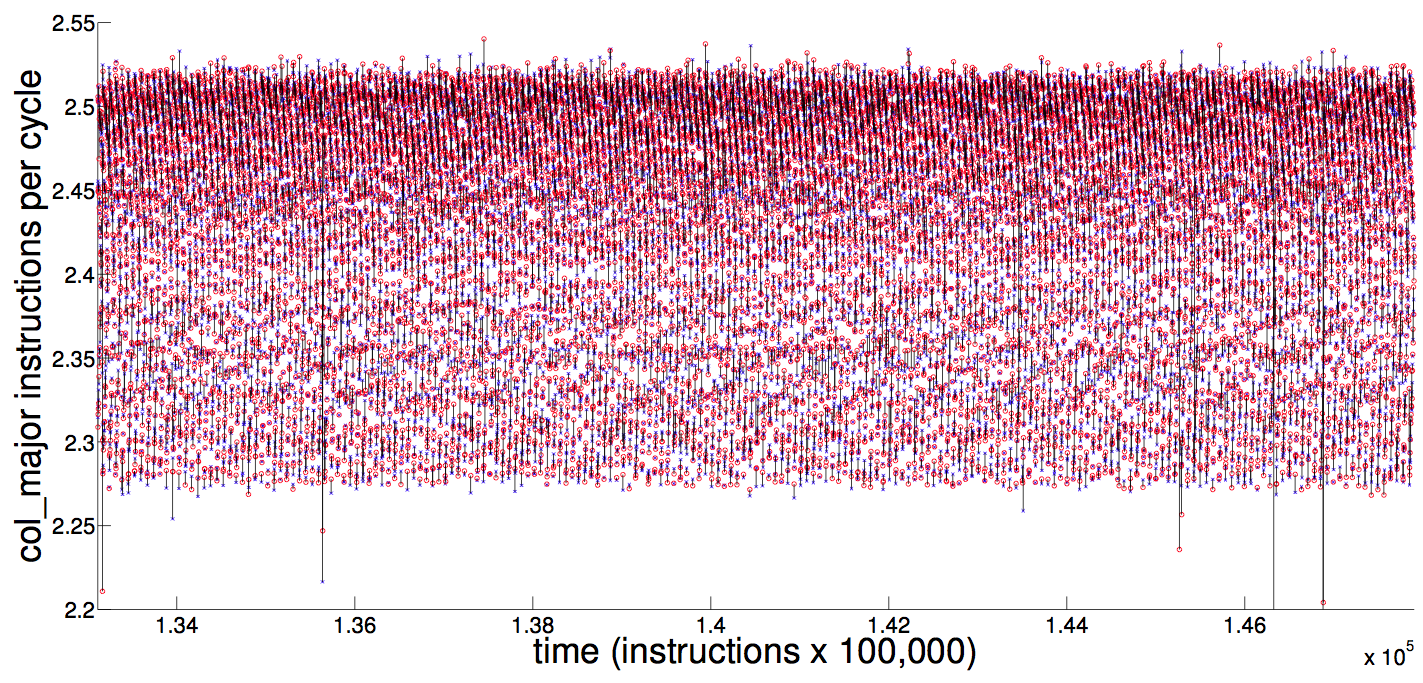
\includegraphics[width=\textwidth]{unused-figs/colPredfullTS}
                \caption{col IPC  Short Time Series for structure illustration}
                \label{fig:svdFullColored}
        \end{subfigure}

        ~ %add desired spacing between images, e. g. ~, \quad, \qquad etc.
          %(or a blank line to force the subfigure onto a new line)
         \caption{col\_major Predictions }\label{fig:svdFull}
\end{figure}



%\begin{figure}[htbp]
%\begin{center}
%\includegraphics[width=\textwidth]{unused-figs/%colPredictionVariation.pdf}
%\end{center}
%\end{figure}






\begin{figure}[htbp]
\begin{center}
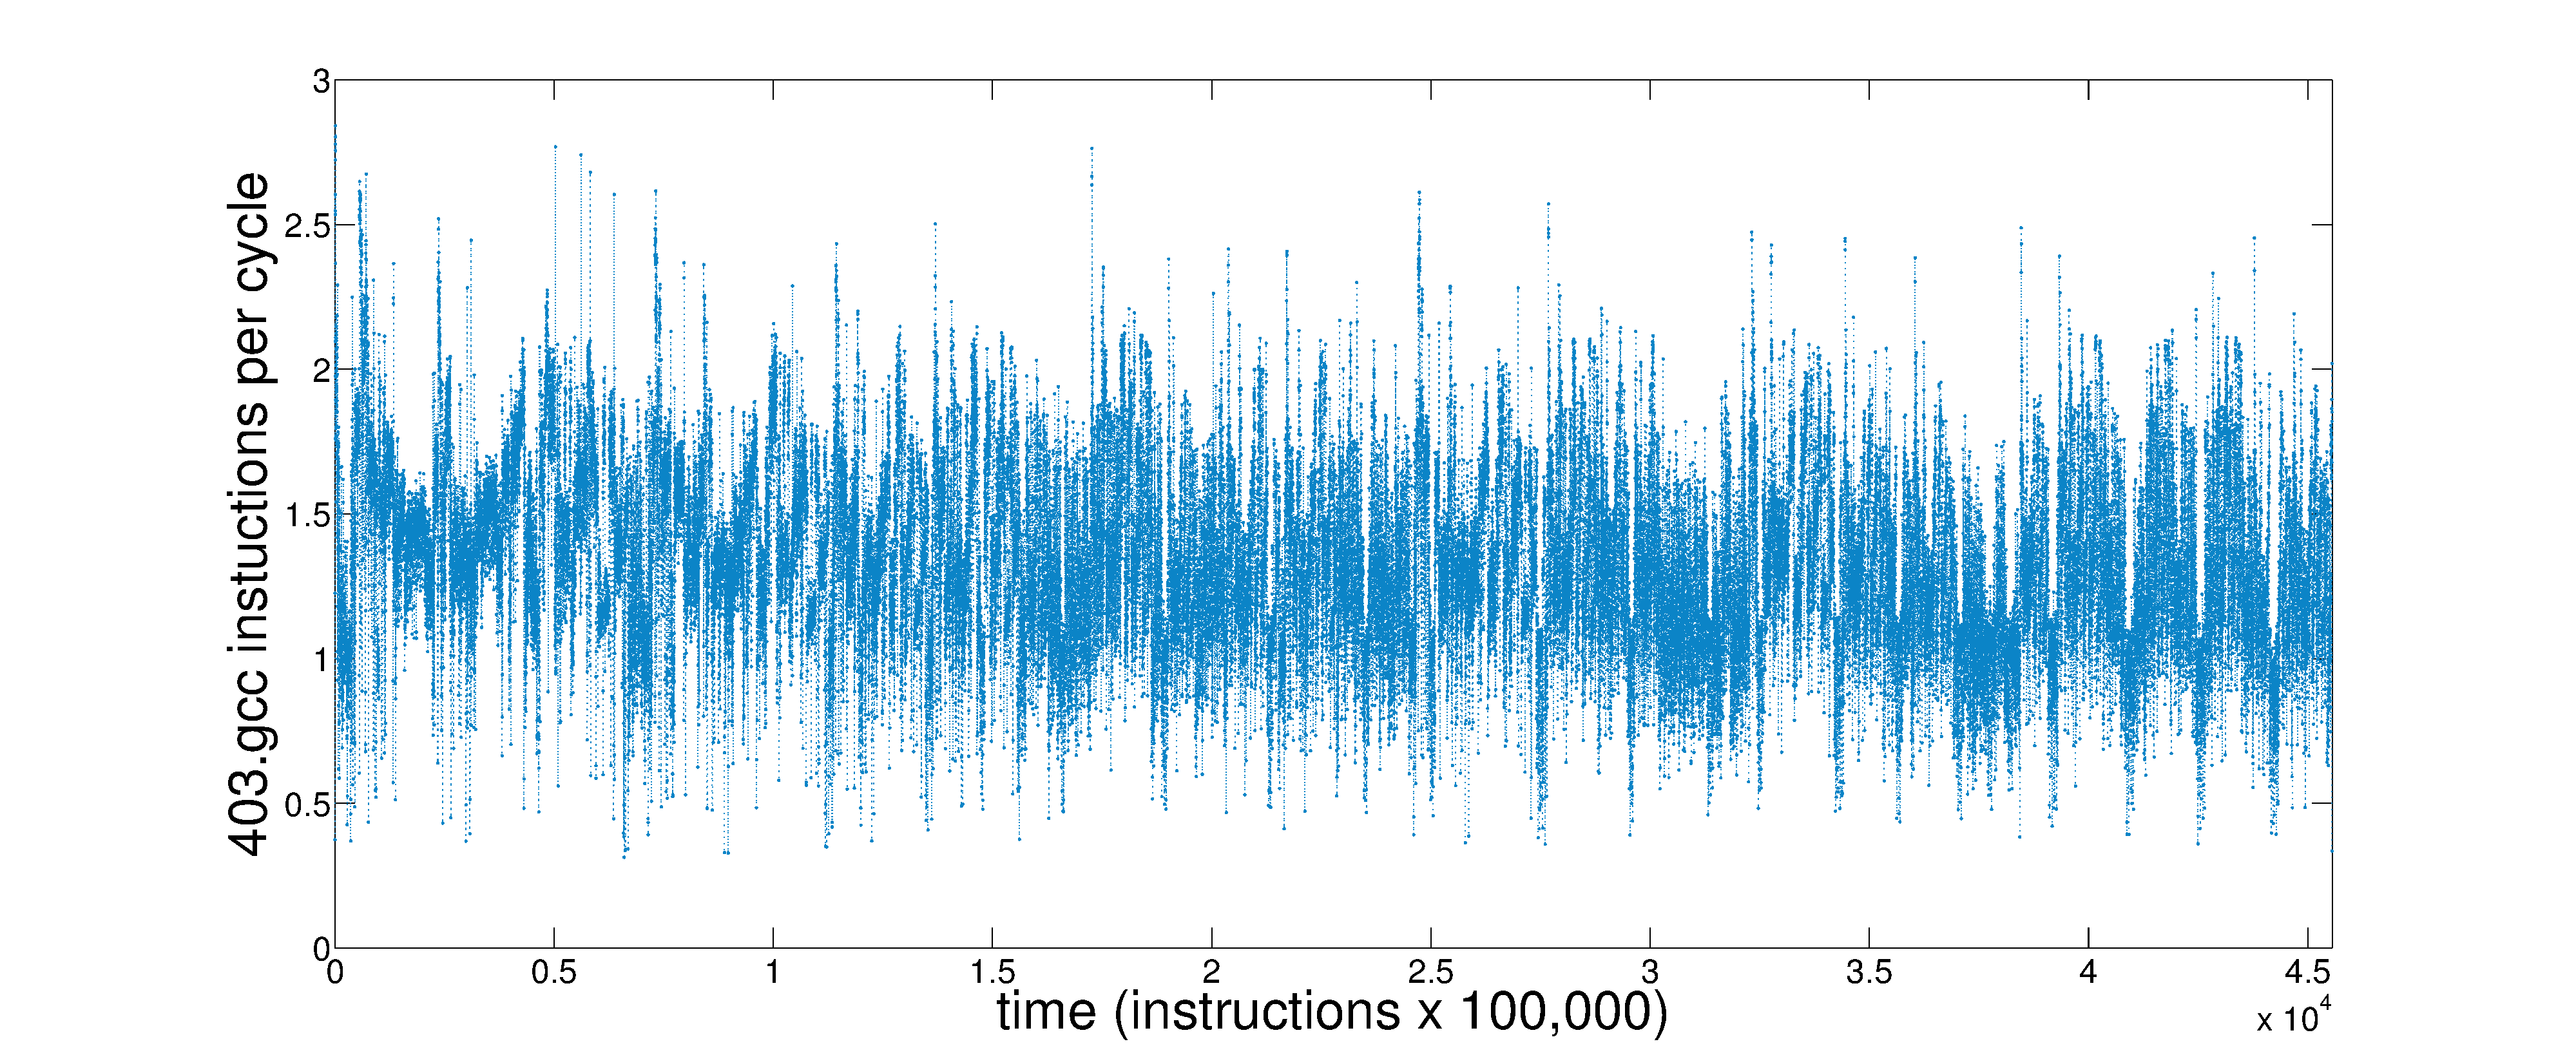
\includegraphics[width=\textwidth]{unused-figs/gccfullts}\caption{403.gcc full time series}
\label{default}
\end{center}
\end{figure}





\begin{figure}[htbp]
\begin{center}
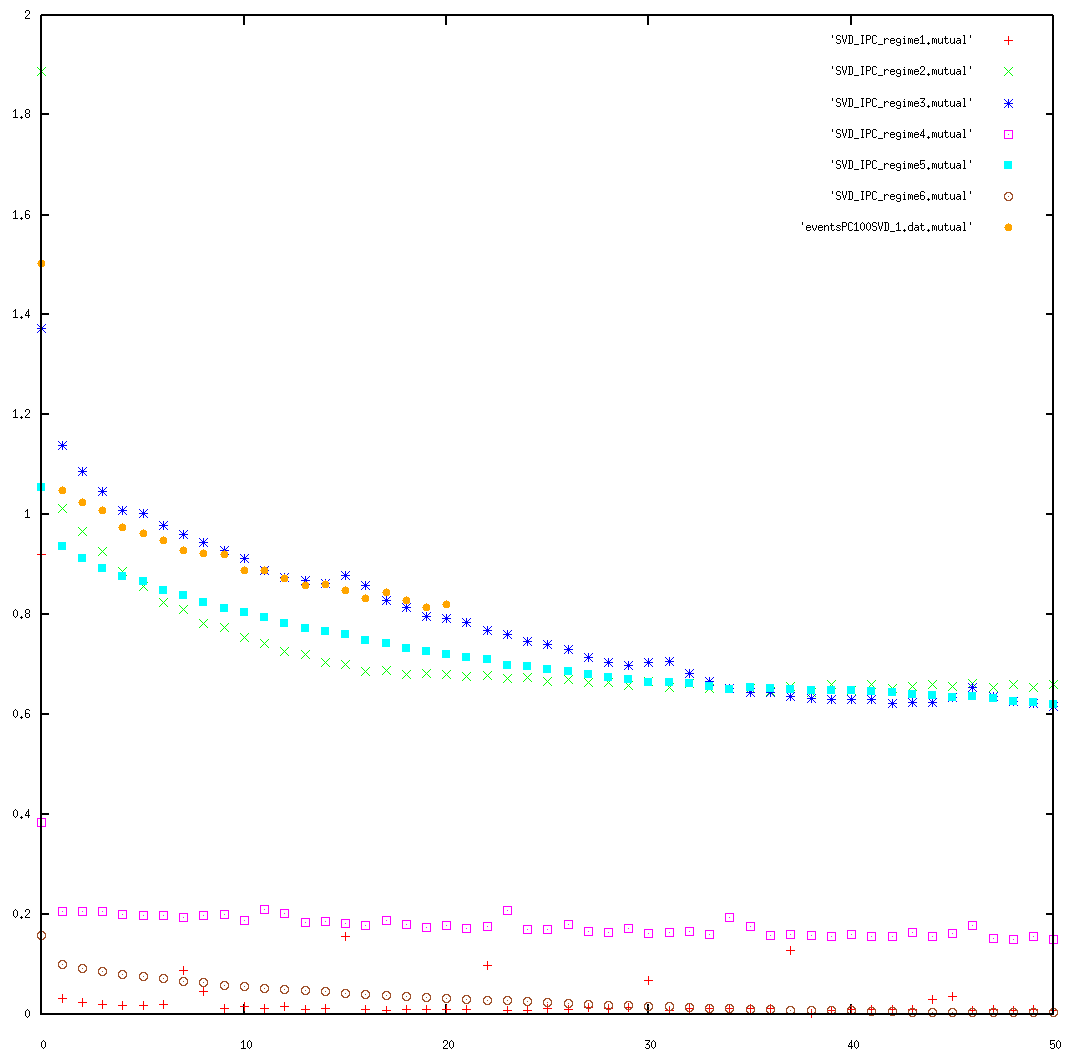
\includegraphics[width=\textwidth]{unused-figs/svd-mutuals}\caption{SVD mutuals for full and regimes}
\label{default}
\end{center}
\end{figure}






\begin{figure}[htbp]
\begin{center}
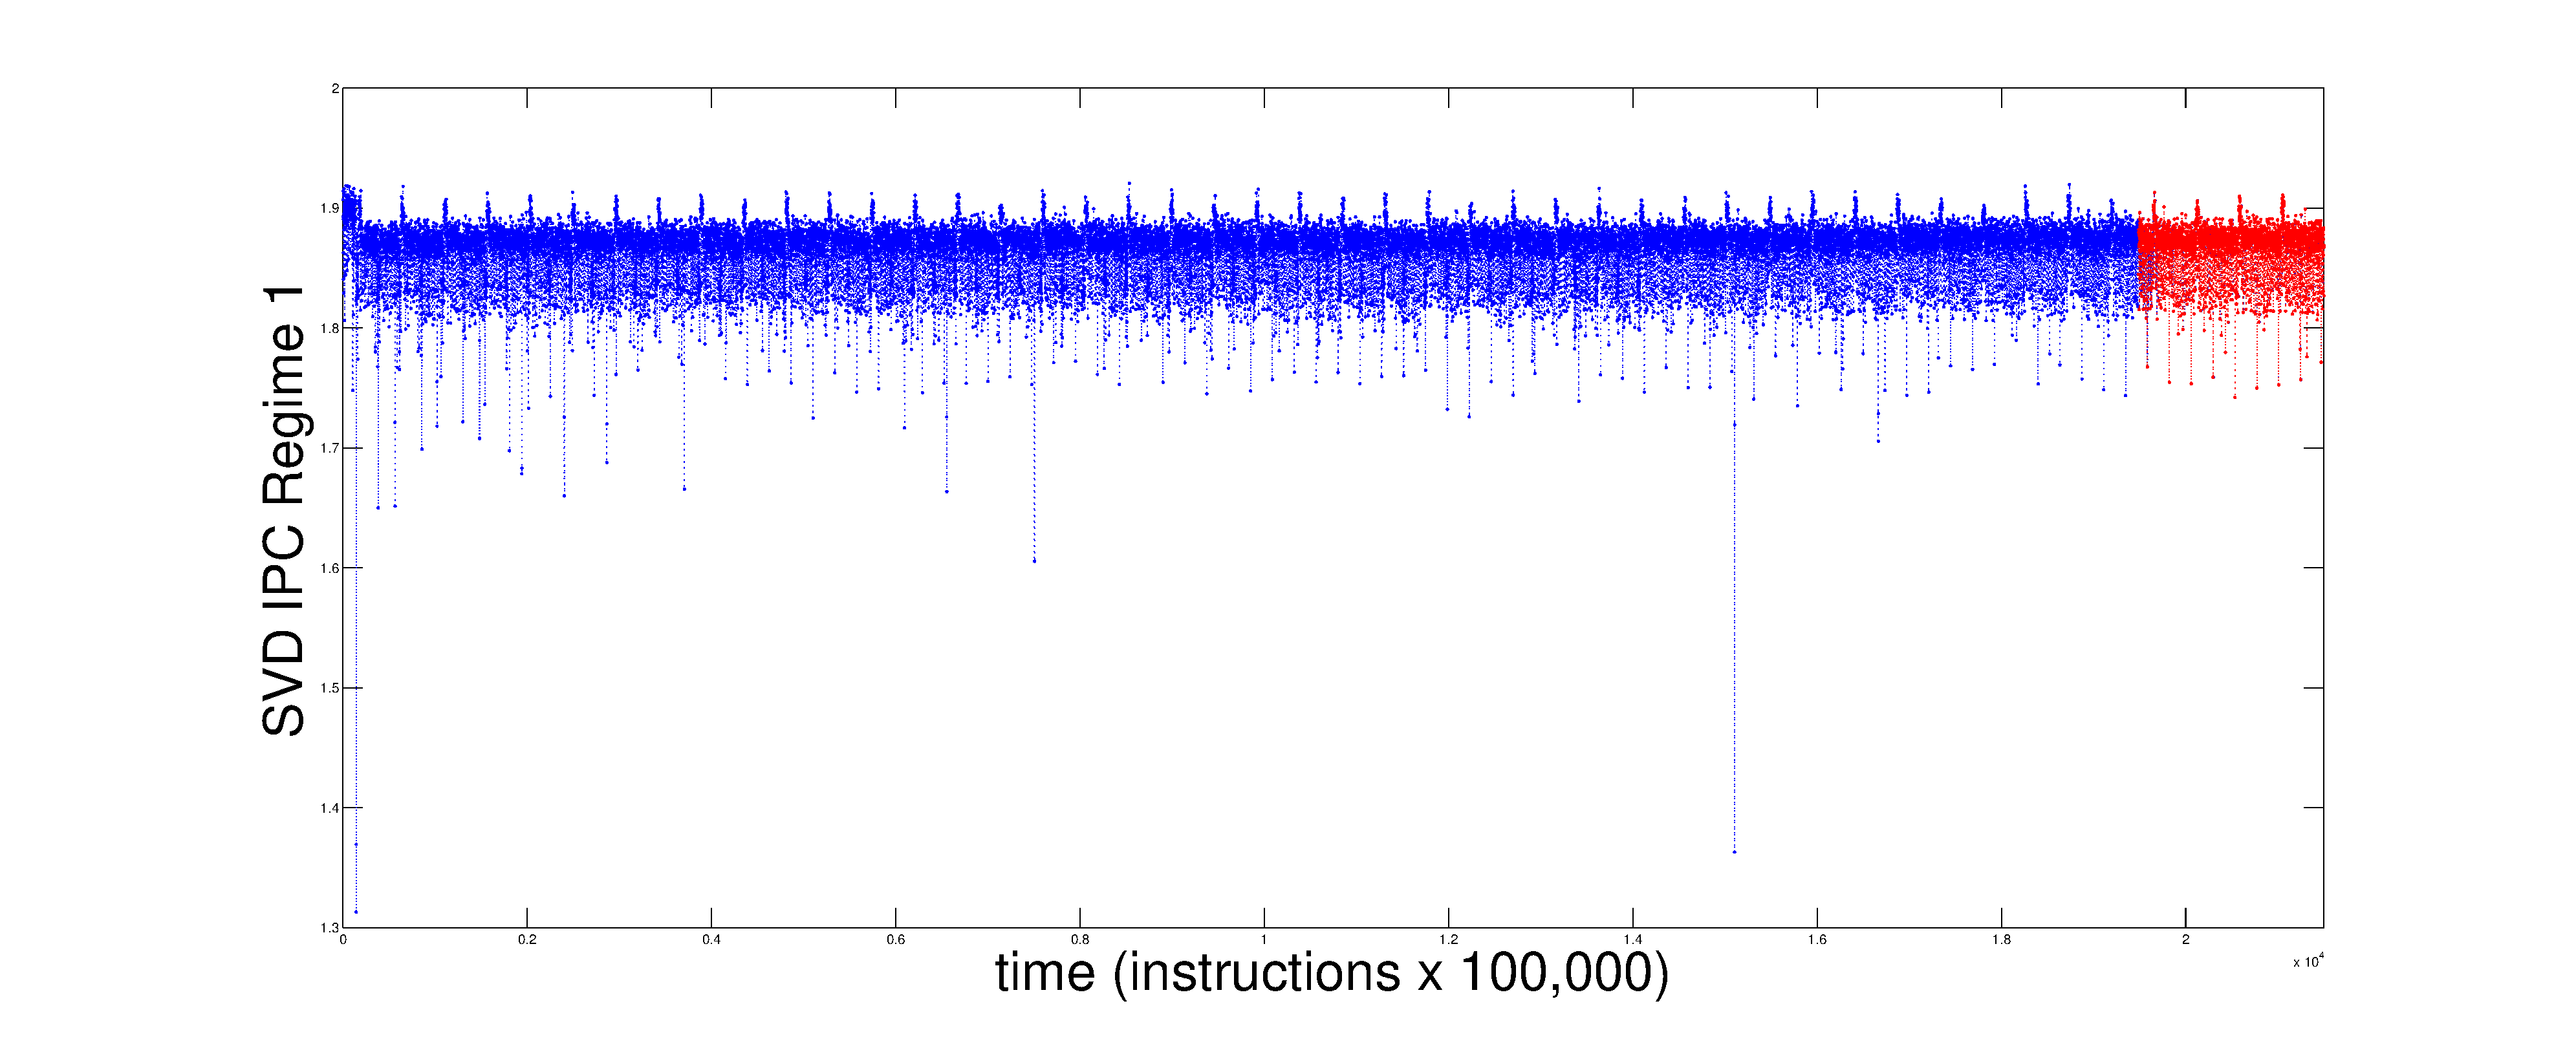
\includegraphics[width=\textwidth]{unused-figs/regime1}\caption{SVD IPC Regime 1 Time Series}
\label{default}
\end{center}
\end{figure}


\begin{figure}[htbp]
\begin{center}
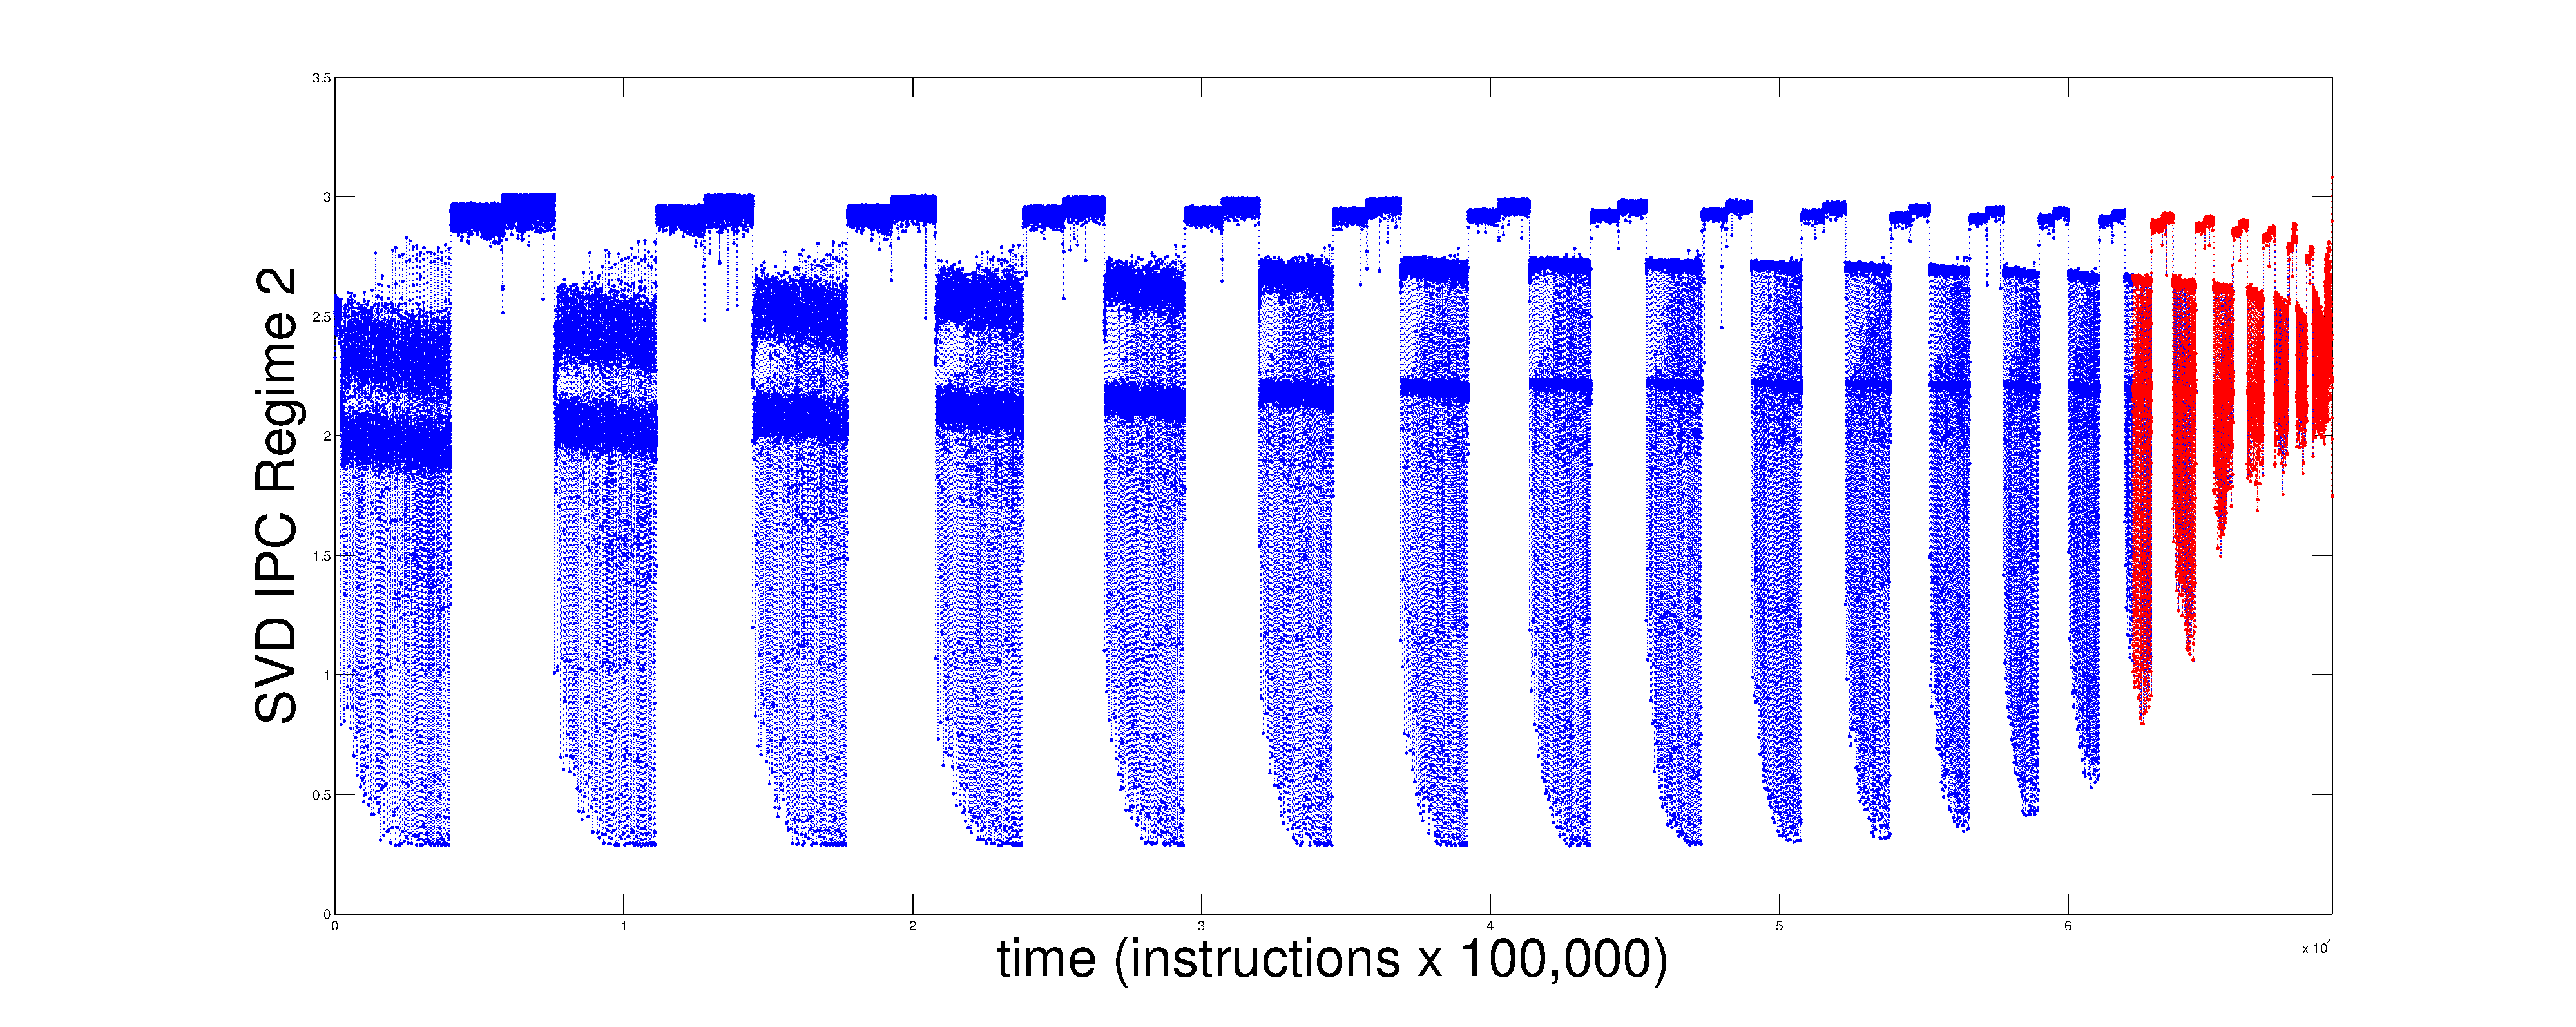
\includegraphics[width=\textwidth]{unused-figs/regime2}\caption{SVD IPC Regime 2 Time Series}
\label{default}
\end{center}
\end{figure}


%\begin{figure}[htbp]
%\begin{center}
%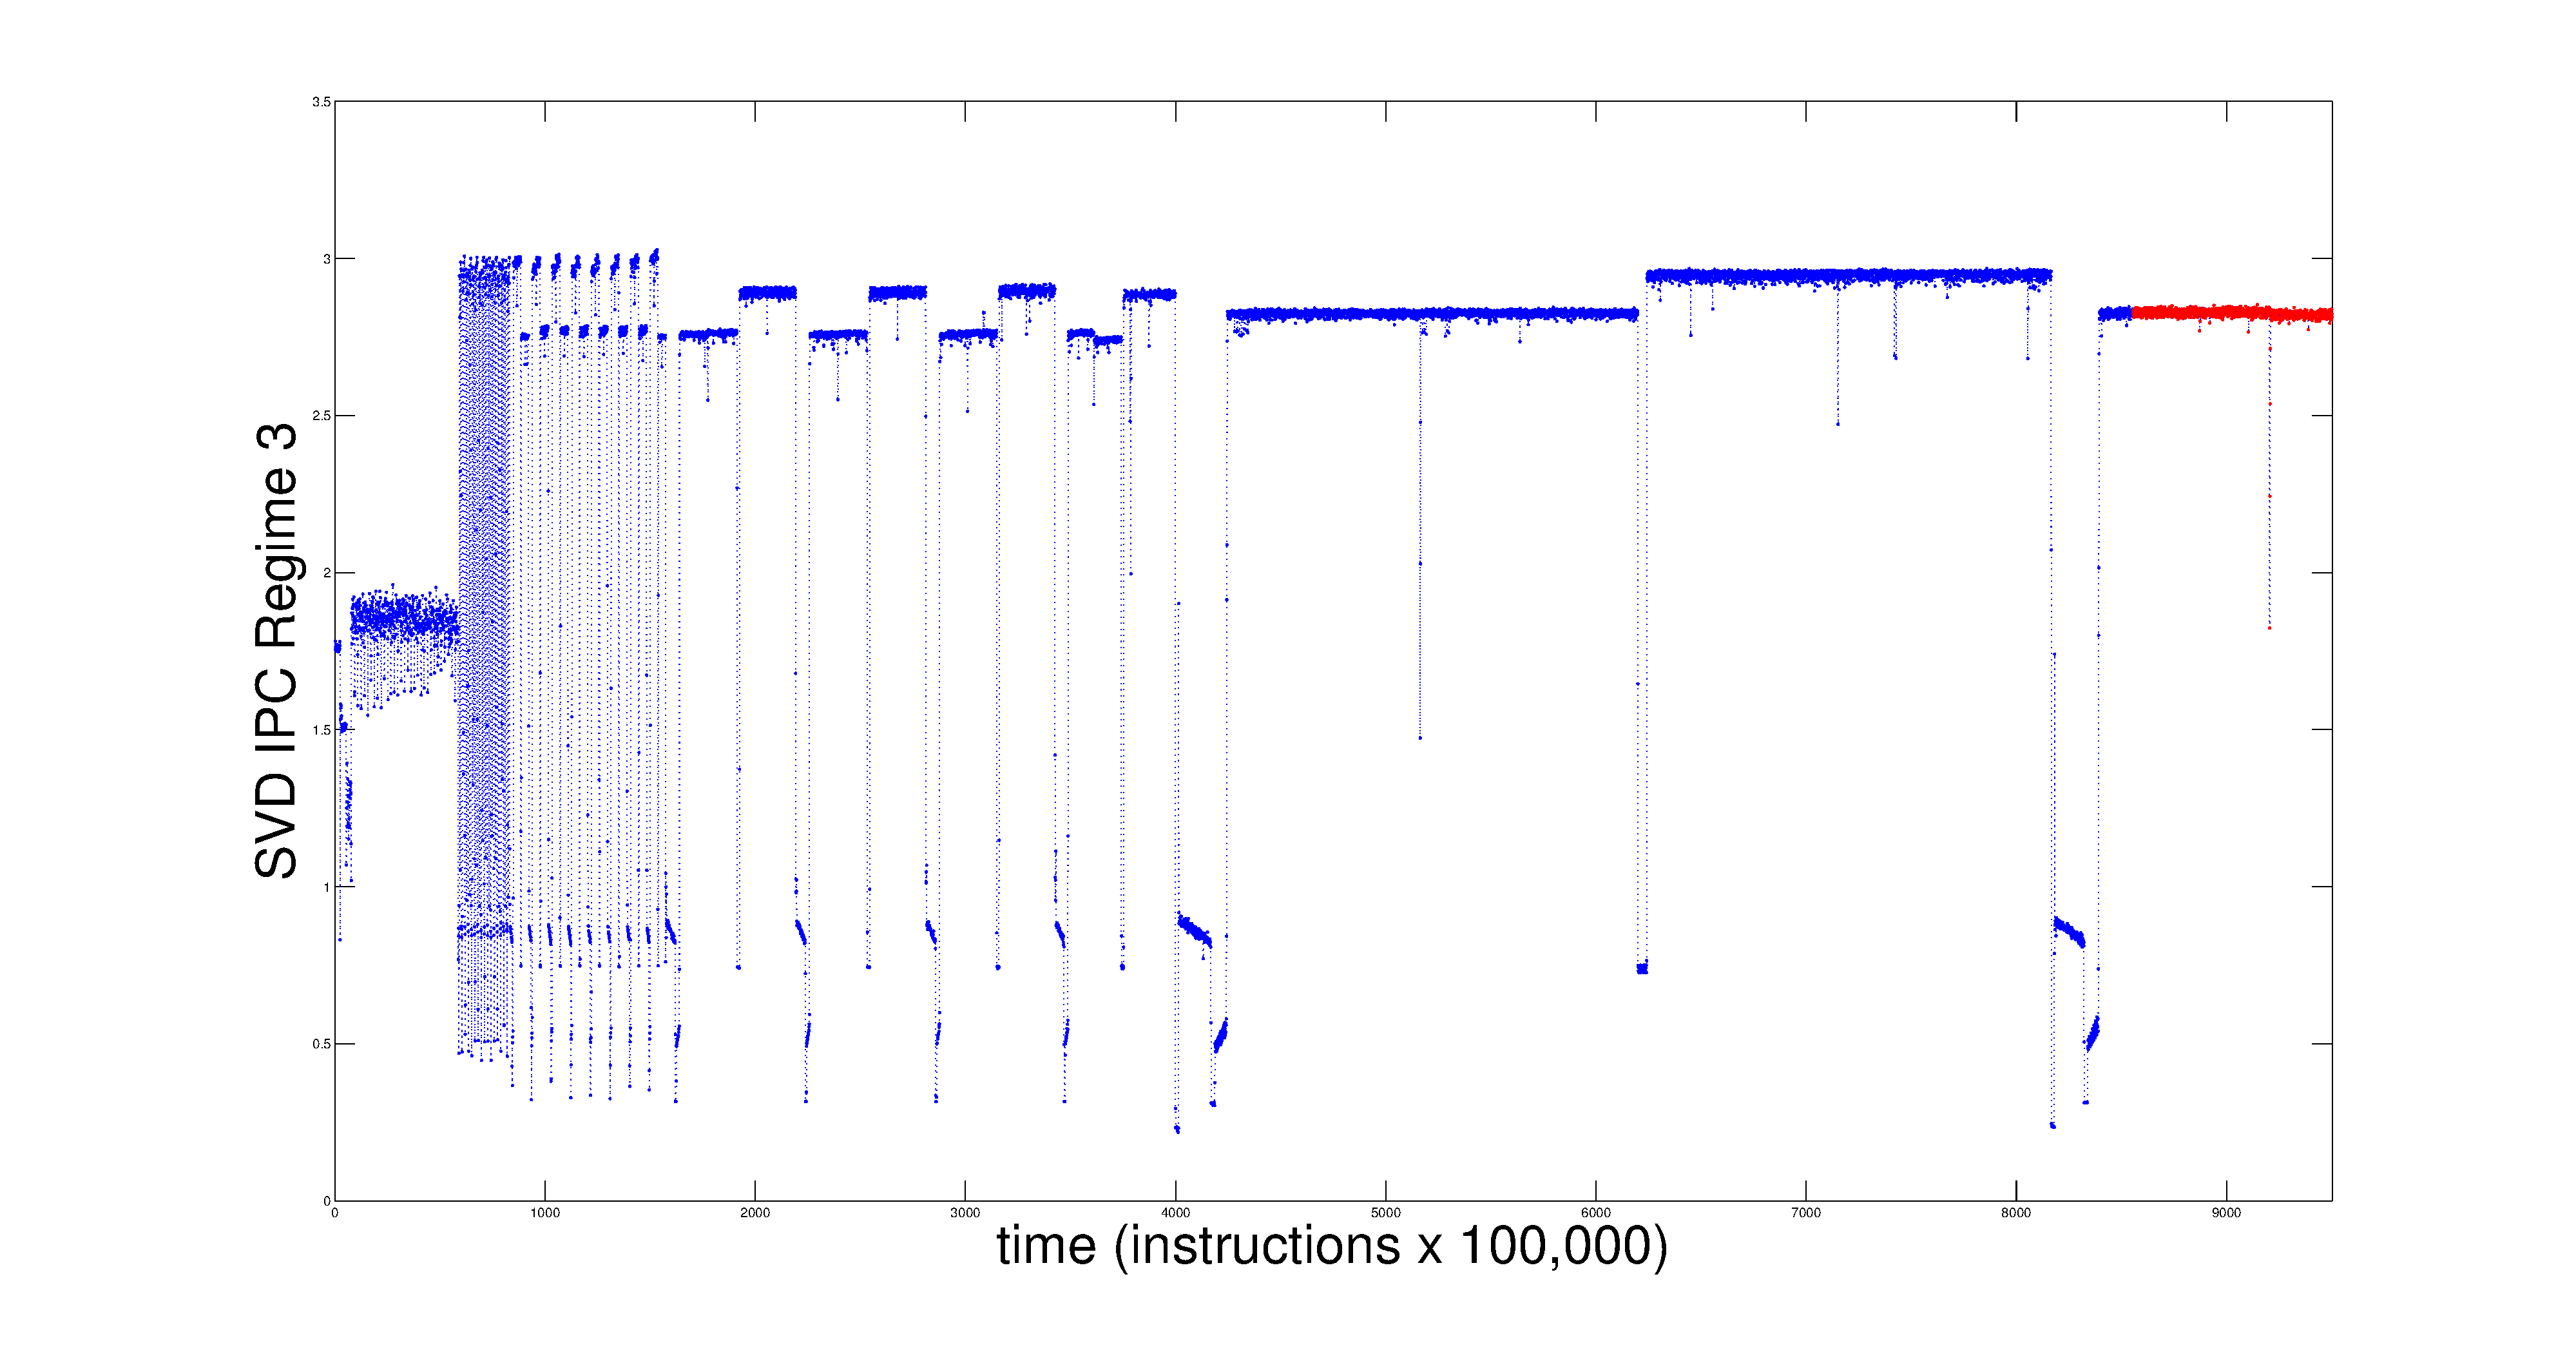
\includegraphics[width=\textwidth]{figs/regime3}\caption{SVD IPC Regime 3 Time Series}
%\label{default}
%\end{center}
%\end{figure}

%\begin{figure}[htbp]
%\begin{center}
%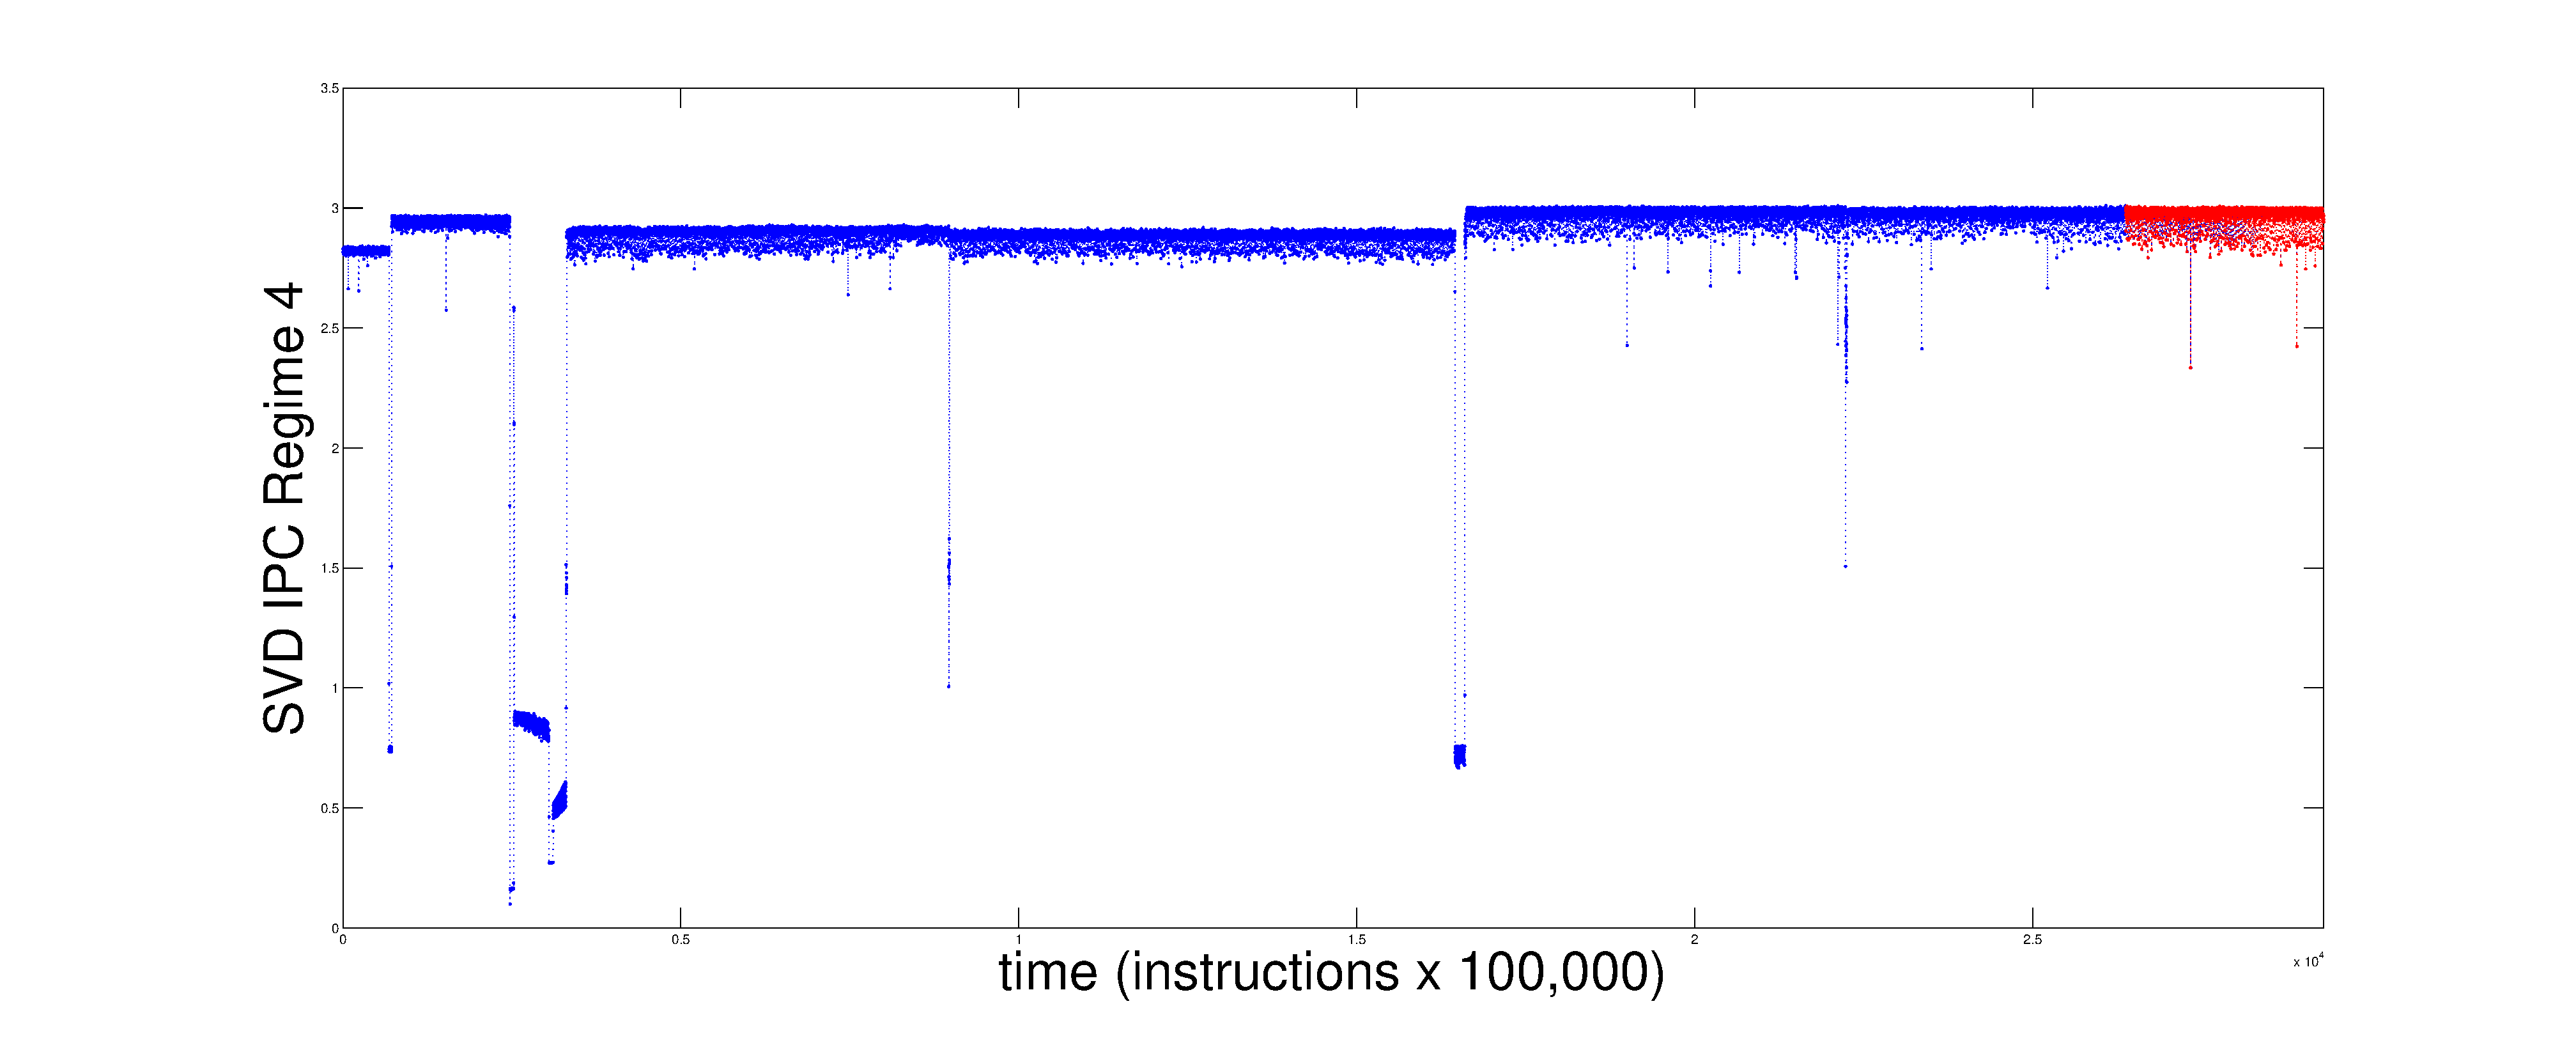
\includegraphics[width=\textwidth]{figs/regime4}\caption{SVD IPC Regime 4 Time Series}
%\label{default}
%\end{center}
%\end{figure}

\begin{figure}[htbp]
\begin{center}
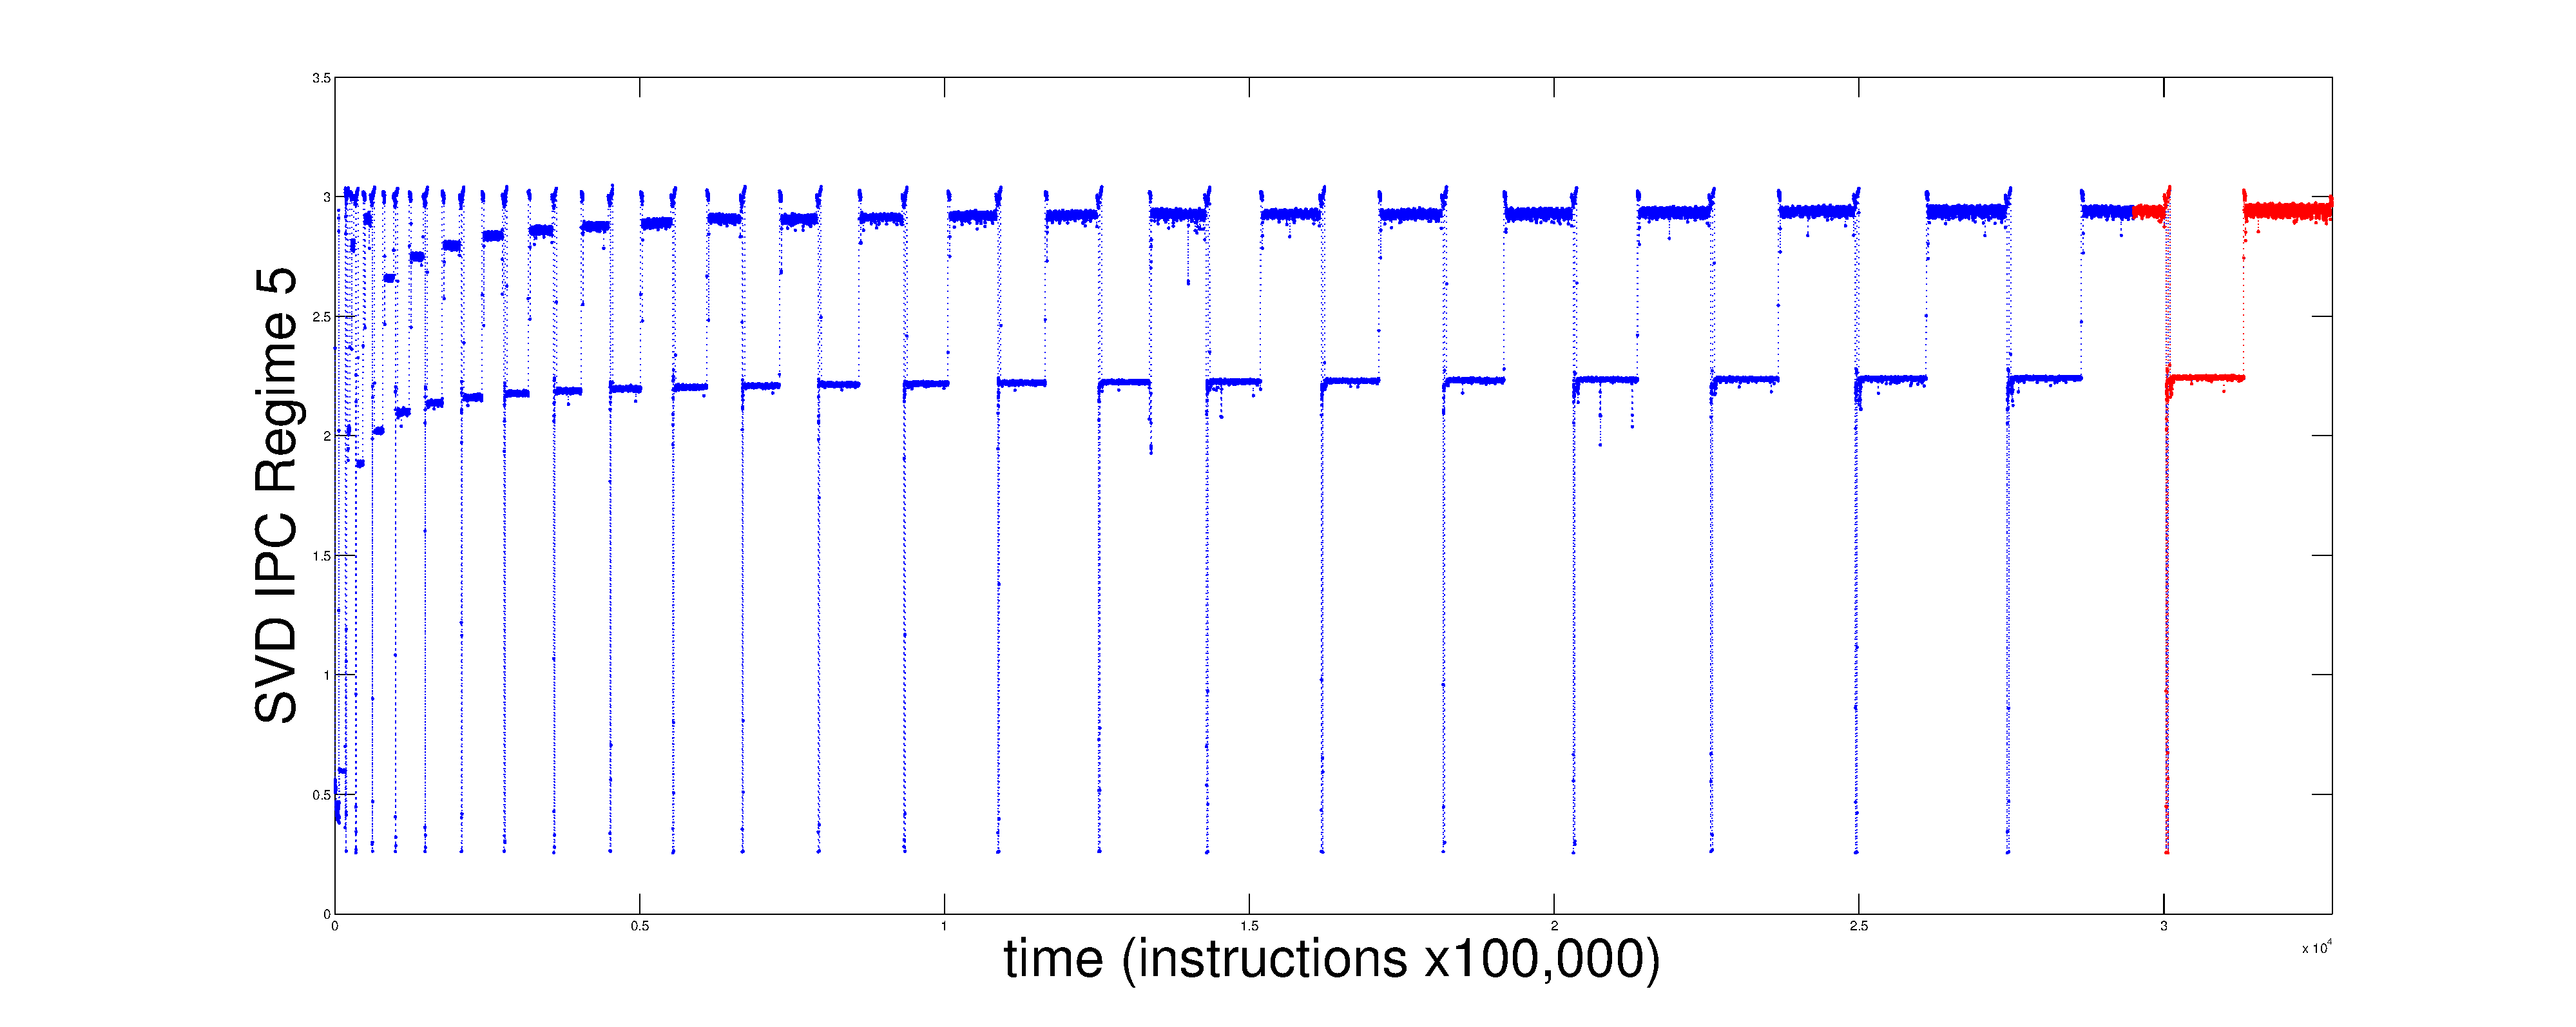
\includegraphics[width=\textwidth]{unused-figs/regime5}\caption{SVD IPC Regime 5 Time Series}
\label{default}
\end{center}
\end{figure}

\begin{figure}[htbp]
\begin{center}
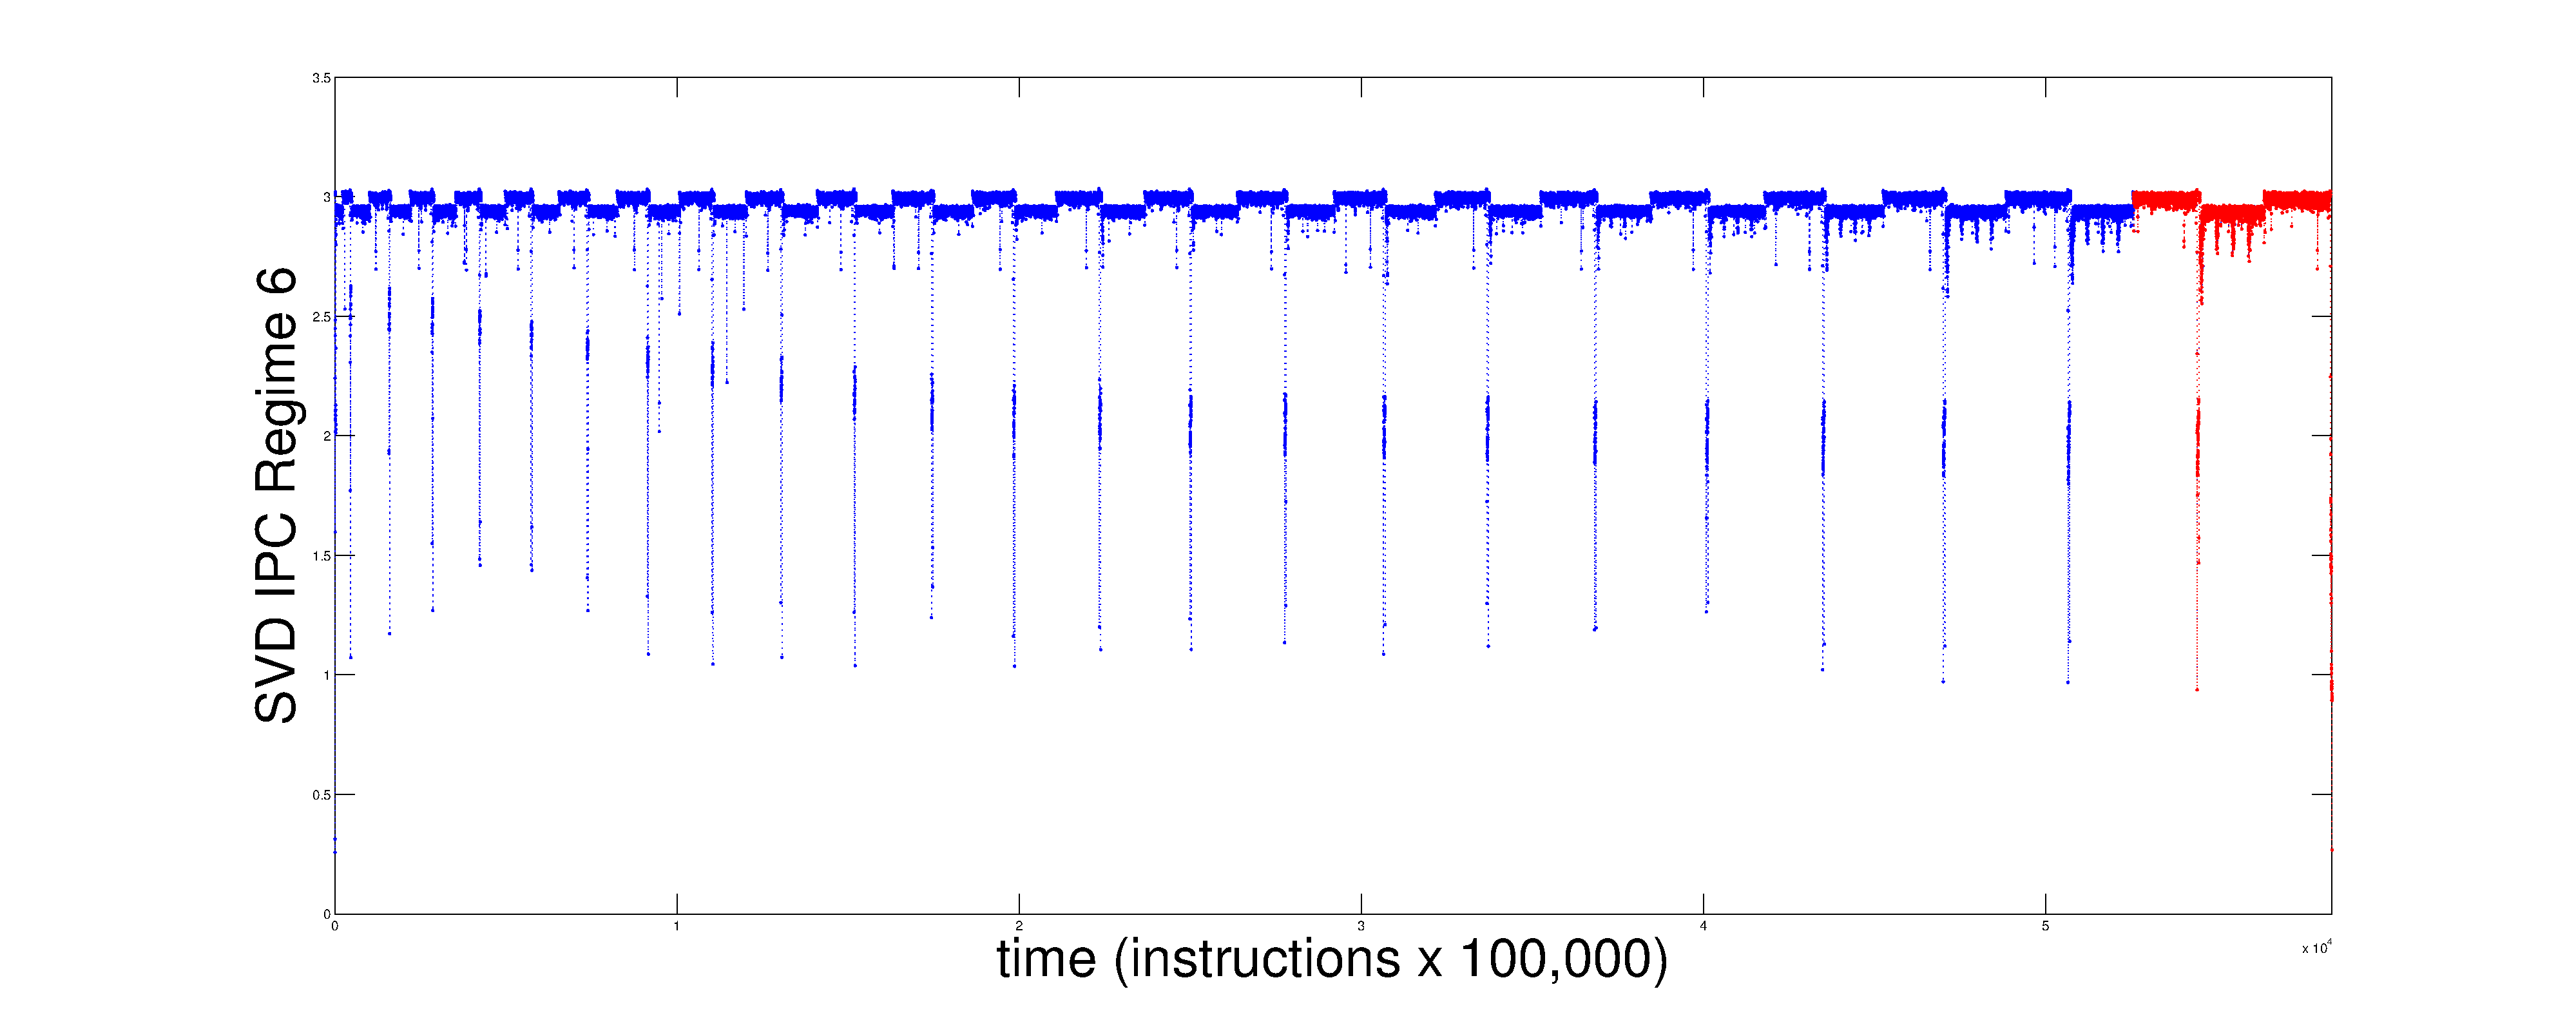
\includegraphics[width=\textwidth]{unused-figs/regime6}\caption{SVD IPC Regime 6 Time Series}
\label{default}
\end{center}
\end{figure}



\section{Unused Tables}


\begin{table}[htdp]
\caption{Average nRMSE over 15 runs for each signal and average wpe at word length 5 and 6 for each signal. }
\begin{center}
\begin{tabular}{|c|c|c|c|c|}
\hline
                   & nRMSE LMA           & nRMSE na\"{i}ve   & $l=5$                   & $l=6$                   \\
\hline
gcc                  & $0.1407 \pm 0.0063$ & $0.1487 \pm 0.0066$ & $0.9510 \pm 0.0011$ & $0.9430 \pm 0.0013$ \\

col\_major          & $0.0252 \pm 0.0061$ & $0.1975 \pm 0.0436$ & $0.5636 \pm 0.0031$ & $0.5131 \pm 0.0034$ \\

SVD\_IPC\_Regime1    & $0.1680 \pm 0.0317$ & $0.3517 \pm 0.5223$ & $0.9761 \pm 0.0084$ & $0.9572 \pm 0.0156$ \\
SVD\_IPC\_Regime2    & $0.1716 \pm 0.0043$ & $0.1762 \pm 0.0012$ & $0.8760 \pm 0.0052$ & $0.8464 \pm 0.0044$ \\
SVD\_IPC\_Regime3      & $0.0507 \pm 0.0011$ & $0.5413 \pm 0.0005$ & $0.7768 \pm 0.0073$ & $0.7157 \pm 0.0056$ \\
SVD\_IPC\_Regime4    & $0.1288 \pm 0.0471$ & $0.2308 \pm 0.0867$ & $0.9073 \pm 0.0080$ & $0.8246 \pm 0.0077$ \\
SVD\_IPC\_Regime5    & $0.0235 \pm 0.0022$ & $0.1306 \pm 0.0003$& $0.7333 \pm 0.0076$ & $0.6776 \pm 0.0068$ \\
SVD\_IPC\_Regime6    & $0.0196 \pm 0.0022$ & $0.0508 \pm 0.0003$ & $0.8101 \pm 0.0135$ & $0.7475 \pm 0.0106$ \\
\hline
\end{tabular}
\end{center}
\label{default}
\end{table}%






\begin{table}[htdp]
\caption{Average nRMSE over 15 runs for each signal and average wpe at word length 5 and 6 for each signal. }
\begin{center}
\begin{tabular}{|c|c|c|c|c|c|c|}
\hline
                  & Horizon & nRMSE LMA           & nRMSE na\"{i}ve           &LMA MASE (ARIMA) & $l=5$                   & $l=6$                   \\
\hline
gcc               & 4,542   & $0.1407 \pm 0.0063$ & $0.1487 \pm 0.0066$ &1.5416(0.929)& $0.9510 \pm 0.0011$ & $0.9430 \pm 0.0013$ \\

col\_major        & 14,709  & $0.0252 \pm 0.0061$ & $0.1975 \pm 0.0436$ &0.0519(0.07UF/0.5740/0.9936)& $0.5636 \pm 0.0031$ & $0.5131 \pm 0.0034$ \\

SVD\_Full         & 22,072  & $0.0323 \pm 0.0019$ & $0.1784 \pm 0.0040$ & $0.8765 \pm 0.0044$ & $0.8508 \pm 0.0035$ \\
SVD\_IPC\_Regime1 & 2,158   & $0.1680 \pm 0.0317$ & $0.3517 \pm 0.5223$ &0.7954(0.724UF)& $0.9761 \pm 0.0084$ & $0.9572 \pm 0.0156$ \\
SVD\_IPC\_Regime2 & 6,902   & $0.1716 \pm 0.0043$ & $0.1762 \pm 0.0012$ &1.9990(1.138)             & $0.8760 \pm 0.0052$ & $0.8464 \pm 0.0044$ \\
SVD\_IPC\_Regime3 & 947     & $0.0507 \pm 0.0011$ & $0.5413 \pm 0.0005$ &1.0089 (1.165215)              & $0.7768 \pm 0.0073$ & $0.7157 \pm 0.0056$ \\
SVD\_IPC\_Regime4 & 2,929   & $0.1288 \pm 0.0471$ & $0.2308 \pm 0.0867$ &0.8976 (0.840548)           & $0.9073 \pm 0.0080$ & $0.8246 \pm 0.0077$ \\
SVD\_IPC\_Regime5 & 3,255   & $0.0235 \pm 0.0022$ & $0.1306 \pm 0.0003$ &0.7487 (1.260/2.3446)& $0.7333 \pm 0.0076$ & $0.6776 \pm 0.0068$ \\
SVD\_IPC\_Regime6 & 5,804   & $0.0196 \pm 0.0022$ & $0.0508 \pm 0.0003$ &0.7848 (0.7831) & $0.8101 \pm 0.0135$ & $0.7475 \pm 0.0106$ \\
\hline
\end{tabular}
\end{center}
\label{default}
\end{table}%














\begin{table}[htdp]
\caption{Average MASE over 15 runs for each signal and average wpe at word length 5 and 6 for each signal. }
\begin{center}
\begin{tabular}{|c|c|c|c|c|c|}
\hline
                   & MASE LMA    & MASE ARIMA &MASE na\"{i}ve & $l=5$  & $l=6$ \\
\hline
gcc                  & $1.9856 \pm $ & $1.7525 \pm $ &1.7904 $\pm$& $0.9510 \pm 0.0011$ & $0.9430 \pm 0.0013$ \\

col\_major           & $ 0.0587\pm $ & $0.9936 \pm $ & $0.5713\pm$& $0.5636 \pm 0.0031$ & $0.5131 \pm 0.0034$ \\




SVD\_IPC\_Regime1     & $ \pm $ & $ \pm $ & $\pm$& $0.9761 \pm 0.0084$ & $0.9572 \pm 0.0156$ \\
SVD\_IPC\_Regime2     & $ 2.3753\pm $ & $0.7268 \pm $ & $3.1064\pm$& $0.8760 \pm 0.0052$ & $0.8464 \pm 0.0044$ \\
SVD\_IPC\_Regime3       & $ \pm $ & $ \pm $ & $\pm$& $0.7768 \pm 0.0073$ & $0.7157 \pm 0.0056$ \\
SVD\_IPC\_Regime4     & $ \pm $ & $ \pm $ & $\pm$&$0.9073 \pm 0.0080$ & $0.8246 \pm 0.0077$ \\
SVD\_IPC\_Regime5     & $4.9079 \pm $ & $2.3366 \pm $ & $21.0372\pm$& $0.7333 \pm 0.0076$ & $0.6776 \pm 0.0068$ \\
SVD\_IPC\_Regime6     & $ \pm $ & $ \pm $ & $\pm$& $0.8101 \pm 0.0135$ & $0.7475 \pm 0.0106$ \\
\hline
\end{tabular}
\end{center}
\label{default}
\end{table}%


\begin{table}[htdp]
\caption{ Embedding Parameters for reference if needed. }
\begin{center}
\begin{tabular}{|c|c|c|}
\hline
&$\tau$ & $m$ \\
\hline
gcc & 10& 13\\
col\_major  &2&12\\
SVD\_Full &  10  &  12 \\
SVD\_IPC\_Regime1 & 5 &14  \\
SVD\_IPC\_Regime2 & 10   &12  \\
SVD\_IPC\_Regime3 & 2   &9  \\
SVD\_IPC\_Regime4 &  3  & 11 \\
SVD\_IPC\_Regime5 &  23  & 10 \\
SVD\_IPC\_Regime6 &  30  & 12  \\
\hline
\end{tabular}
\end{center}
\label{default}
\end{table}%

 Table~\ref{tab:pe} shows the permutation entropy results for the
 examples considered in this paper, with the nRMSPE prediction
 accuracies from the previous section included alongside for easy
 comparison.

 \begin{table}[htbp]
   % increase table row spacing, adjust to taste
   \renewcommand{\arraystretch}{1.3}
   \caption{TCM NRMSE and PE NORMS}
   \label{tab:table_example}
   \centering
   % Some packages, such as MDW tools, offer better commands for making tables
   % than the plain LaTeX2e tabular which is used here.
   \begin{tabular}{|c|c|c|c|c|c|}
     \hline
     TCM & NRMSE & $m=3$  &$m=4$&$m=5$&$m=6$\\
     \hline
     \tt{row\_major} & 0.0102 & 0.7900  &0.6751&0.5458&0.4491\\
     \hline
     \tt{col\_major} & 0.0055 & 0.6411  &0.5029&0.4515&0.3955 \\
     \hline
     \tt{403.gcc} & 0.0865 & 0.9954  &0.9916&0.9880&0.9835\\
     \hline
     \tt{482.sphinx3} & 0.1142 & 0.9958  &0.9913&0.9866&0.9802 \\
      \hline
   \end{tabular}
 \end{table}

%  \begin{table}[htbp]
%   % increase table row spacing, adjust to taste
%   %\renewcommand{\arraystretch}{1.3}
%   \caption{Cache-miss rate performance traces: prediction error
%     (nRMSPE) and permutation entropy}
%   \label{tab:TCMpe}
%   \centering
%   % Some packages, such as MDW tools, offer better commands for making tables
%   % than the plain LaTeX2e tabular which is used here.
%   \begin{tabular}{|c|c|c|c|c|c|}
%     \hline
%      & nRMSE   &$n=4$&$n=5$&$n=6$\\
%     \hline
%     \tt{row\_major}  & 0.0324  &0.6751&0.5458&0.4491\\
%     \hline
%     \tt{col\_major}  & 0.0080  &0.5029&0.4515&0.3955 \\
%     \hline
%     \tt{403.gcc}  & 0.1416  &0.9916&0.9880&0.9835\\
%     \hline
%     \tt{482.sphinx3}  & 0.2032  &0.9913&0.9866&0.9802 \\
%      \hline
%   \end{tabular}
% \end{table}

 \begin{table}[htbp]
   % increase table row spacing, adjust to taste
   \renewcommand{\arraystretch}{1.3}
   \caption{IPC NRMSE and PE NORMS}
   \label{tab:table_example}
   \centering
   % Some packages, such as MDW tools, offer better commands for making tables
   % than the plain LaTeX2e tabular which is used here.
   \begin{tabular}{|c|c|c|c|c|c|}
     \hline
     ipc & NRMSE & $n=3$  &$n=4$&$n=5$&$n=6$\\
     \hline
      \tt{row\_major} & 0.0095 & 0.9912  &0.9723&0.9354&0.8876\\
     \hline
      \tt{col\_major} & 0.0071 & 0.9428  &0.8356&0.7601&0.6880\\
     \hline
     \tt{403.gcc} & 0.1805 & 0.9918  &0.9862&0.9814&0.9764\\
     \hline
     \tt{482.sphinx3} & 0.2946 & 0.9978  &0.9951&0.9914&0.9849 \\
      \hline
   \end{tabular}
 \end{table}

%  \begin{table}[htbp]
%   % increase table row spacing, adjust to taste
%   %\renewcommand{\arraystretch}{1.1}
%   \caption{Processor load performance traces: prediction error
%     (nRMSPE) and permutation entropy}
%   \label{tab:IPCpe}
%   \centering
%   % Some packages, such as MDW tools, offer better commands for making tables
%   % than the plain LaTeX2e tabular which is used here.
%   \begin{tabular}{|c|c|c|c|c|}
%     \hline
%      & nRMSPE   &$n=4$&$n=5$&$n=6$\\
%     \hline
%      \tt{row\_major} & 0.0778  &0.9723&0.9354&0.8876\\
%     \hline
%      \tt{col\_major} & 0.0161   &0.8356&0.7601&0.6880\\
%     \hline
%     \tt{403.gcc} & 0.2033   &0.9862&0.9814&0.9764\\
%     \hline
%     \tt{482.sphinx3} & 0.3670 & 0.9951&0.9914&0.9849 \\
%      \hline
%   \end{tabular}
% \end{table}

 %  \begin{table}[htbp]
 %   \caption{Prediction error (in nRMSPE) and permutation entropy (for
 %     different wordlengths $n$}
 %   \label{tab:pe}
 %   \centering
 %   \begin{tabular}{|c|c|c|c|c|c|}
 %     \hline
 %      {\bf cache misses} & error   &$n=4$&$n=5$&$n=6$\\
 %     \hline
 %     \tt{row\_major}  & 0.0324  &0.6751&0.5458&0.4491\\
 %     \hline
 %     \tt{col\_major}  & 0.0080  &0.5029&0.4515&0.3955 \\
 %     \hline
 %     \tt{403.gcc}  & 0.1416  &0.9916&0.9880&0.9835\\
 %     \hline
 %     \tt{482.sphinx3}  & 0.2032  &0.9913&0.9866&0.9802 \\
 %      \hline
 %      \hline
 %      {\bf insts per cyc} & error   &$n=4$&$n=5$&$n=6$\\
 %     \hline
 %      \tt{row\_major} & 0.0778  &0.9723&0.9354&0.8876\\
 %     \hline
 %      \tt{col\_major} & 0.0161   &0.8356&0.7601&0.6880\\
 %     \hline
 %     \tt{403.gcc} & 0.2033   &0.9862&0.9814&0.9764\\
 %     \hline
 %     \tt{482.sphinx3} & 0.3670 & 0.9951&0.9914&0.9849 \\
 %      \hline
 %   \end{tabular}
 % \end{table}


  \begin{table}[htbp]
   % increase table row spacing, adjust to taste
   \renewcommand{\arraystretch}{1.3}
   \caption{Normalized root mean squared error (nRMSE) of 4000-point
     predictions of memory \& processor performance from different
     programs.}
   \label{tab:PredError}
   \centering
   % Some packages, such as MDW tools, offer better commands for making tables
   % than the plain LaTeX2e tabular which is used here.
%   \begin{tabular}{|c|c|c|c|c|c|}
%     \hline
%      & cache misses NRMSE & IPC NRMSE \\
%     \hline
%     \tt{row\_major}  & 0.0102  & 0.0095 \\
%          \hline
%     \tt{col\_major}  &0.0055& 0.0071 \\
%     \hline
%     \tt{403.gcc}  & 0.0865& 0.1805 \\
%          \hline
%     \tt{482.sphinx3} & 0.1142& 0.2946 \\
%      \hline
%   \end{tabular}
% \end{table}
   \begin{tabular}{|c|c|c|c|c|c|}
     \hline
      & cache miss rate & instrs per cycle \\
     \hline
     \tt{row\_major}  & 0.0324  & 0.0778 \\
          \hline
     \tt{col\_major}  &0.0080& 0.0161 \\
     \hline
     \tt{403.gcc}  & 0.1416& 0.2033 \\
          \hline
     \tt{482.sphinx3} & 0.2032& 0.3670 \\
      \hline
   \end{tabular}
 \end{table}




\section{Unused Text}
%****BEYOND THIS POINT IS A DIFFERNT PAPER*** JOSHUA WILL CLEAN THIS OUT, JUST HERE FOR REFERNCE****
\section{Introduction: What is Permutation Entropy}


%\begin{it}
%Here I want to talk about the definition and algorithm for computing it. Maybe briefly talk about the asymptotic %properties. (i.e., same as metric topological in limit. Converges to dominate leap if not normalized etc. )
%\end{it}

When analyzing a time series there are several standard characterizations of complexity, including (but not limited to) entropy, Lyapunov exponents and fractal dimensions. Rigorous definitions of all these quantities exist if the observation is a \emph{noise-free} trajectory of a \emph{single} dynamical system. To an experimental-time-series analyst these are luxuries that are rarely (if ever) realized. Many times experimental observation have noise involved such as sensor error, or very commonly in the computer world finite-precision error.

Unfortunately the standard algorithms for calculating many of these complexity measures are highly sensitive to noise and give spurious results in the presence of noisy observations. Even worse, if a time-series observation measures multiple dynamical systems or dynamical systems that undergo bifurcations\footnote{A drastic change in the behavior of the dynamical system, generally associated with parameter drift.} then all of the standard algorithms for estimating complexity, (e.g., correlation dimension) go out the window. Bandt and Pompe first introduced \emph{permutation entropy} as a ``natural complexity measure for time series" in 2002 \cite{bandt2002per}.


As explained in \cite{bandt2002per}, permutation entropy is a simple complexity measure that is easily calculated for any time series, be it stochastic, periodic, quasi-periodic, chaotic, noisy or any combination of these. Most importantly for analysis of computer performance, permutation entropy as defined in \cite{bandt2002per} yields meaningful results even if observational or dynamical noise is present \cite{bandt2002per}.




Analyzing entropies as  a complexity measure is not a new concept, however the way that the entropy is estimated in \cite{bandt2002per} is novel and particularly useful when little is known about the underlying process.   As discussed in \cite{bandt2002per}, the standard entropy one considers is Shannon entropy.


As a quick review of Shannon entropy, we follow the treatment in \cite{amigo2012permutation}. Given a finite alphabet $\mathcal{S} = \{s_1,....,s_{|\mathcal{S}|}\}$, define an information source as a discrete-time, stationary stochastic process $X = \{X_n\}_{n \in \mathbb{N}_0}$ where $X_n$ are random variables on a common probability space taking on values from $\mathcal{S}$. A realization of $X$ is a one-sided sequence $x_0^{\infty} = (x_n)_{n \in \mathbb{N}_0}$ called a \emph{message}. The elements $x_n$ of $\mathcal{S}$ are the \emph{symbols}(a.k.a letters) of the language. A finite segment of the message, say $x_k^{k+m-1} = x_kx_{k+1} \dots x_{k+m-1}$ is called a \emph{word} (of length m). We then define $p(x_0^{m-1})$ to be the probability of the word $x_0^{m-1}$ to appear some where in the message. The shannon entropy of the data source $X$ is defined as: \begin{equation}\label{eq:shannonentropy}
h(X) = - \lim_{m\to\infty}\frac{1}{m}\sum p(x_0^{m-1})\log p(x_0^{m-1})
\end{equation}

For the purposes of this paper once can view entropy as a measure of complexity and predictability in a time series. A high entropy almost completely unpredictable and a small entropy is completely predictable. This spectrum is outlined very nicely in \cite{amigo2012permutation}: ``Periodic or quasiperiodic sequences have vanishing or negligible complexity. At the opposite end, independent and identically distributed random sequences (white noise) have asymptotically divergent permutation entropies, owing to the fact that the number of allowed (or ``admissible�?) ordinal patterns grows superexponentially with length. Between both ends lie the kind of sequences we are interested in."

This illustrates why utilizing entropy as a measure for complexity is, in theory, a great candidate. There are several fundamental drawbacks with this approach when analyzing real-world time series. The two most fundamental problems are as follows:

\begin{enumerate}
\item Elements of an experimental time series $x_t \in \mathbb{R}$ which implies $x_t \notin \mathcal{S}$, for a finite alphabet $\mathcal{S}$.
\item Time series are always finite in length so the limit in \ref{eq:shannonentropy} never exists in practice.
\end{enumerate}


The common practice to address item 1 is to perform \emph{symbolization} on the time series you want to analyze. Symbolization is the process of defining a dynamic preserving map $\phi: \mathbb{R}^m \to \mathcal{S}$, i.e., for each $x_t$ (or block $x_k^{k+m-1} = x_kx_{k+1} \dots x_{k+m-1}$) we must assign a symbol from $\mathcal{S}$ in such a way that the time series has the same fundamental properties.  There are several approaches to symbolization, the standard approach is partitioning. Assume, $x_t$ has the capability of taking on infinitely many values, defining the space $X$ to be the space where these $x_t$ are drawn. We then define a partition on this space $X = P_1 \cup...\cup P_m$, and define $\mathcal{S} = \{1,\dots,m\}$. Then $\phi(x_t) = i$ if $x_t \in P_i$. We can then calculate the Shannon entropy of the transformed time series, which in the limit of $m$ converges to the Kolmogorov-Sinai entropy \cite{bandt2002per}. This approach to symbolization is computationally infeasable as we need an infinite number of partitions of an infinite time series. For \emph{extremely} rare cases, there exists a \emph{generating} partition where this limit is not necessary. However, finding such a partition even for a simple two-dimensional map like Henon is non-trivial \cite{bandt2002per}. Finding a generating partition for an arbitrary time series is for all intensive purposes impossible.

[[[Maybe also talk about Mischaikow's approach to this with isolating neighborhoods and homology...but might be off topic. ]]]


.....



Instead of this approach to symbolization, Bandt et al. take the approach that ``the symbol sequence must come naturally for the time series, without any further model assumptions" \cite{bandt2002per}. To do this they perform symbolization through ordinal analysis. Ordinal analysis of a time series is the process of mapping the ordered successive elements of a time series to a permutation of the same size based on their original time-based ordering.[[Need a better way of wording this]]. This is also referred to in the literature as the permutation complexity \cite{amigo2012permutation}  For example, if $(x_1,x_2,x_3) = (9,1,7)$ then $\phi$ maps $(x_1,x_2,x_3)$ to the permutation $231$ since $x_2 < x_3<x_1$. A great explanation of why this is an interesting symbolization is found in \cite{amigo2012permutation} :

\begin{quote}The study of permutation complexity, which we call ordinal analysis, can be envisioned as a new kind of symbolic dynamics whose basic blocks are ordinal patterns. Interesting enough, it turns out that under some mild mathematical assumptions, not all ordinal patterns can be materialized by the orbits of a given one- or multi-dimensional deterministic dynamics, not even if this dynamic is chaotic�? contrarily to what happens with the symbol patterns. As a result, the existence of �?forbidden�? (i.e., not occurring) ordinal patterns is always a persistent dynamical feature, in opposition to properties such as proximity and correlation which die out with time in a chaotic dynamic. Moreover, if an ordinal pattern is forbidden, its absence pervades all longer patterns in form of more missing ordinal patterns, called outgrowth forbidden patterns. Admissible ordinal patterns grow exponentially with length, while forbidden patterns do superexponentially. Since random (unconstrained) dynamics has no forbidden patterns with probability 1, their existence can be used as a fingerprint of deterministic orbit generation.
\end{quote} Essentially by analyzing the permutation entropy of a time series we are gaining information as to the complexity of the system without any other information available, whether the time series is generated by a random process or the trajectory of a deterministic dynamical system. Now that we have justified why the study of permutation entropy is interesting let us define it. For this we follow \cite{bandt2002per}.


\begin{mydef}[Permutation Entropy]
Given a time series $\{x_t\}_{t = 1,\dots,T}$. Define $\mathcal{S}_n$ as all $n!$ permutations $\pi$ of order $n$. For each $\pi \in \mathcal{S}_n$ we determine the relative frequency of that permutation occurring in $\{x_t\}_{t = 1,\dots,T}$: \begin{equation}\label{eq:permprob}
p(\pi) = \frac{|\{t|t\le T-n,\phi(x_{t+1},\dots,x_{t+n}) = \pi\}|}{T-n+1}\end{equation}
Where $|\cdot|$ is set cardinality. The \emph{permutation entropy} of order $n\ge 2$ is defined as $$H(n) = - \sum_{\pi \in \mathcal{S}_n} p(\pi)\log_2p(\pi)$$ Notice that $0\le H(n) \le \log_2(n!)$,\cite{bandt2002per}. With this in mind, it is common in the literature to present permutation entropy normalized, i.e., $\frac{H(n)}{\log_2(n!)}$. With this convention, \emph{low} entropy is close to 0 and \emph{high} entropy is entropy close to 1.
\end{mydef}

Notes: According to \cite{bandt2002per} equation (\ref{eq:permprob}) estimates the frequency of $\pi$ as good as possible for a finite series of values. To determine $p(\pi)$ exactly, we have to assume an infinite time series and take the limit as $T\to \infty$ in (\ref{eq:permprob}). Bandt et al., also point out that this limit exists under a very weak stationarity condition: for $k\le n$, the probability for $x_t<x_{t+k}$ should not depend on $t$.

It should also be noted that this is discrete-metric (or shannon) permutation entropy, to be distinguished from topological permutation entropy (a.k.a. permutation capacity). Topological permutation entropy is defined in \cite{amigo2012permutation} as: $$h(\{x_t\}_{t = 1,\dots,\infty}) =  \lim_{L\to\infty}\frac{1}{L}logN(L)$$ where $N(L)$ is the number of distinct ordinal patterns that occur of order $L$. This is a measure of how many distinct permutations of length $L$ are realized as opposed to counting the frequency at which each occurs as is the case in metric permutation entropy \cite{amigo2012permutation}. It can be shown that metric and topological entropy both converge to the true value with probability 1 in the limit.  (citation for this). When we say permutation entropy in this paper we are referring to that defined in \ref{eq:permprob}.



\section{Possible Applications to Computer Systems Performance}


\begin{enumerate}
\item In this section I want to discuss the symbolization of performance traces and why this is advantageous over generating partitions and similar approaches.
\item No model is assumed, some traces do appear to be stochastic some appear to be deterministic this provides ``proof" thereof. albeit not mathematical proof but CS proof for sure.
\item We have essentially infinite data. So limits like $m!$ where $m$ is word length isn't really an issue for us.
\end{enumerate}


\subsection{Predictability and model change detection}

Talk about how some explanatory models may be spinning their wheels because no transferable information. That is if you are introducing pure entropy at every time step really no use in using past values and statistically the mean is the most accurate.

\begin{enumerate}
\item Comp Performance goes under constant bifurcations. This allows autonomous detection of when a model is no longer valid. (need to be careful here with use of valid as to not be confused with model validation.
\item Maybe can tell us if we should use a linear-stochastic, nonlinear-deterministic model or just guess the mean
\end{enumerate}


\begin{figure}[ht]
  \centering
  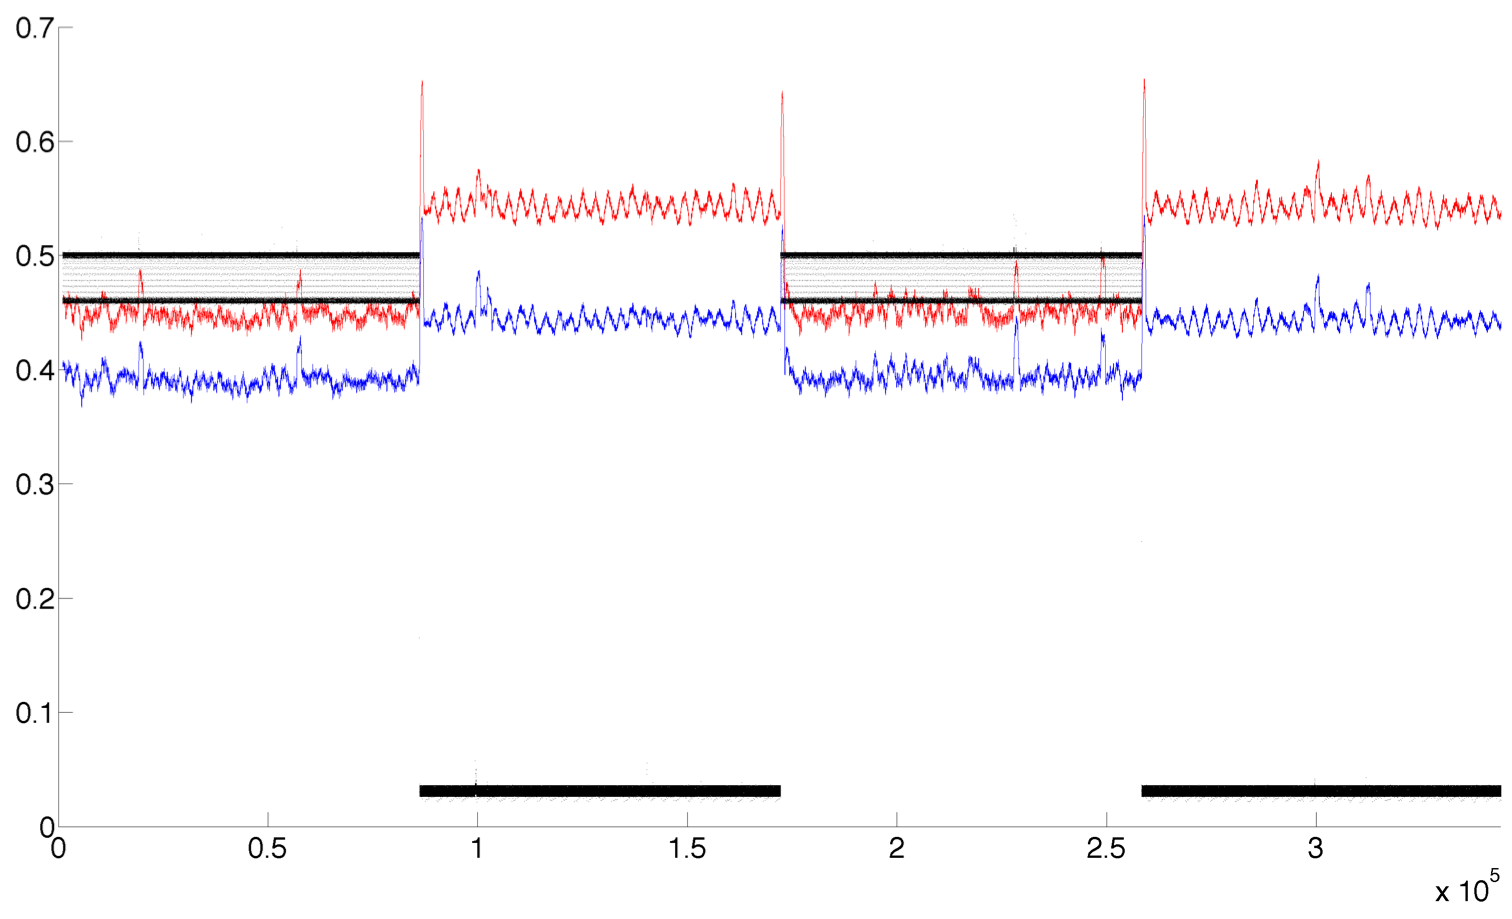
\includegraphics[width=\columnwidth]{unused-figs/ts-rowcol-pe}
  \caption{A time series of cache misses during the execution of the row-col microkernel. The red and blue curves are permutation entropy calculated using $\tau =1$ and $m=5,6$ (respectively). }\label{fig:rowcol}
\end{figure}


\begin{figure}[ht]
  \centering
  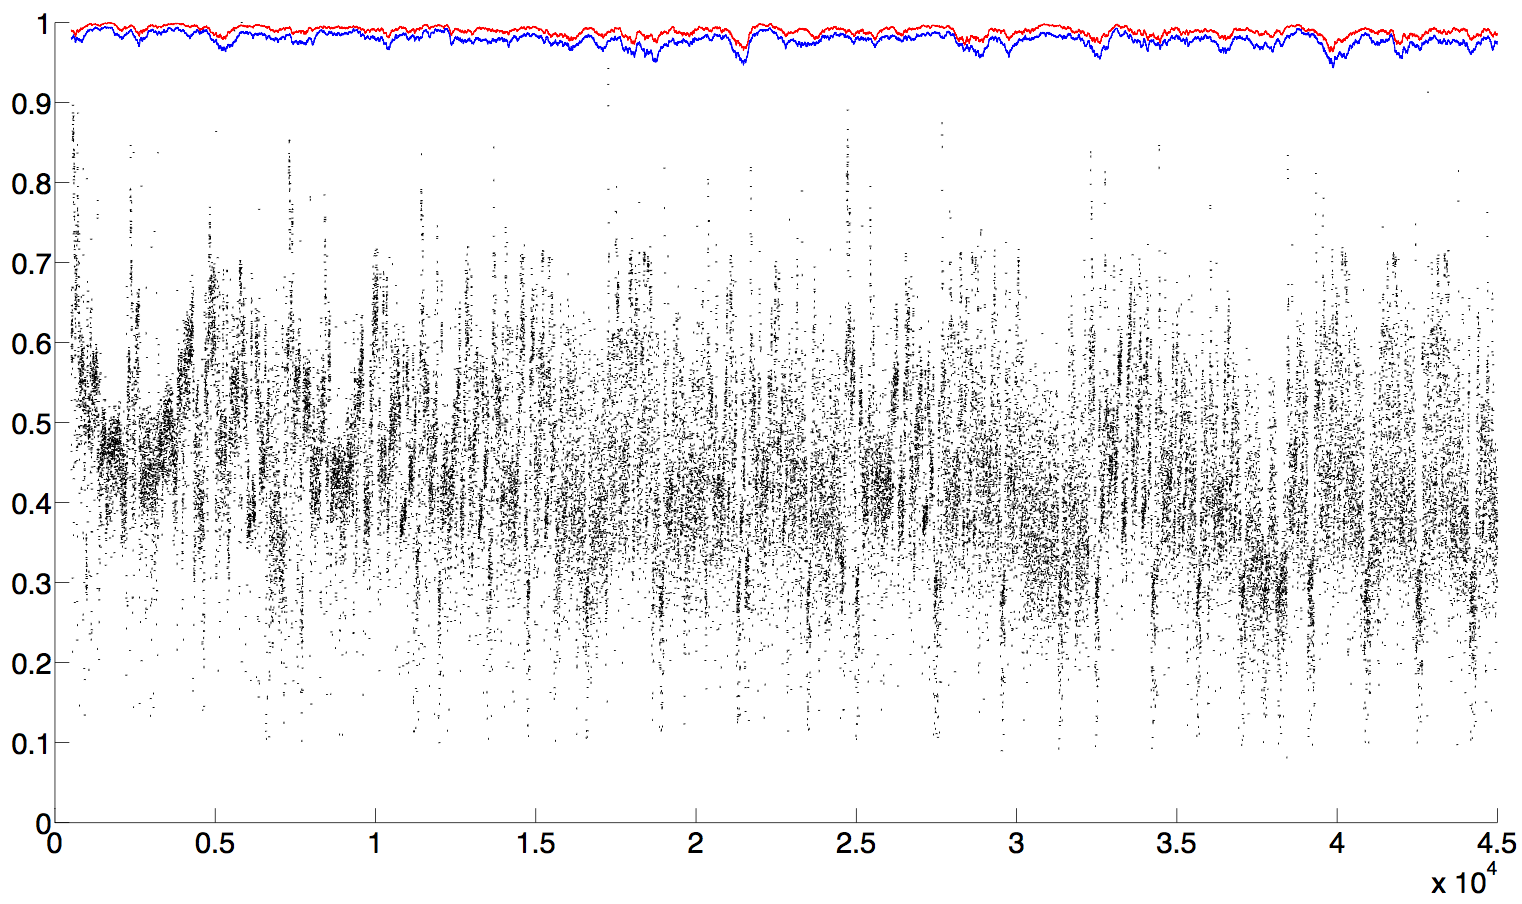
\includegraphics[width=\columnwidth]{unused-figs/ts-gcc-pe}
  \caption{A time series of instructions per cycle for the gcc spec benchmark. The red and blue curves are permutation entropy calculated using $\tau =1$ and $m=3,4$ (respectively). The lack of structure in such a signal illustrates that the use of deterministic models is most likely not the most advantageous.}\label{fig:gcc}
\end{figure}



\section{Pro and Cons}
\subsection{Advantages of Permutation Entropy}
Permutation entropy allows for symbolization of a time series without any further assumptions being made about the underlying system. In fact, virtually nothing needs to be known before applying this techniques. Other methods of symbolization require expert knowledge of the underlying system, such as generating partitions. These techniques have been applied to small data sets, this is truly an advantage especially when dealing with a lot of biological systems whose large datasets can be in the tens of thousands. The algorithm for computing permutation entropy is very straight forward and easy to explain. The actual code takes longer than I would like to run, but this seems to be an issue with my implementation and not the algorithm, as others state they have exceptionally fast algorithms. Although none of these algorithms are ever provided in the literature. The major advantages of permutation entropy is that it can quickly give us a rough estimate of where drastic changes in the time series which may have implications in model selection techniques. Permutation entropy also can give you a quick idea about if a system has deterministic structure. This has direct implications on what prediction strategies to implement.
%\begin{enumerate}
%\item Allows for symbolization without a model. Really emphasize we can obtain a symbolization without generating partitions which is the traditional approach here.
%\item Small amounts of data not really a problem.
%\item Maybe talk about how much data is needed per word length for results that mean anything.
%\item Fairly easy to calculate, although need a more efficient method.
%\item Gives a rough estimation of where drastic changes have occurred in a TS
%\item Allows you to see if there is actually something predictable in the signal.
%\end{enumerate}

\subsection{Disadvantages of PE}
There are three disadvantages with permutation entropy we can immediately see that need further thought to be overcome. The first is that it is sometimes hard to tell when a change in the dynamical system is not drastic enough to have a huge change on the entropy. For example, consider a dynamical system switching from a chaotic to a (different) chaotic regime. The permutation entropy may be very similar while the model is slightly different. Permutation entropy seems to be ill-suited for fine grain detection of this nature. Our current implementation is too slow for on-the-fly analysis. We do not believe this is an issue with permutation entropy itself but with our implementation. The literature all claims that fast algorithms exist.

The biggest disadvantage for us in using permutation entropy is selection of parameters. To calculate permutation entropy, we have to choose an embedding dimension, a lag, and a block size. In all the literature we have found thus far, parameter selection is made based on persistence or matching the permutation entropy to known values. The problem comes when analyzing real time series these parameters seem to have a real impact on the results. Finding (or creating) a rigorous method for parameter selection is paramount in the use of this method for the analysis of real world time series.
%\begin{enumerate}
%\item Paramaters!
%\item Currently numerically expensive although the literature disagrees. Think this might just be my implementation. Need to read the numerics section of the PE book.
%\item Sometimes hard to tell a regime shift has occurred if the transition is chaotic to chaotic. or low period to low period.
%\end{enumerate}

%[[Joshua: It may be interesting to look at the PE as a function of
%prediction horizon. It is known to me that certain start and end
%locations in the prediction strategy result in different prediction
%accuracy. Is it the case that when the algorithm tanks it is also the
%case that PE of the **TEST**(the 10\% we cut off )is high? This may
%be a great way to illustrate the concept if it works... OR maybe do
%complexity of forward path in embedding space?]]  some notes about
%this looking at row Cache 1000 very good RMSPE 21.4167 m = 3 4 5 6
%1.4192 2.1286 2.5942 2.9230 row Cache 2000 very good RMSPE 19.0990 m
%= 3 4 5 6 1.4145 2.1305 2.5825 2.9095 so even better row Cache 2010
%RMSPE 19.9716 m = 3 4 5 6 1.4149 2.1311 2.5830 2.9096 row Cache 1990
%RMSPE 19.1465 So prediction Horizons ranked in order of best RMSPE
%RMSPE L 3 4 5 6 1st 19.0990 2000 1.4145 2.1305 2.5825 2.9095 2nd
%19.1465 1990 1.4151 2.1293 2.5803 2.9067 3rd 19.9716 2010 1.4149
%2.1311 2.5830 2.9096 3rd 21.4167 1000 1.4192 2.1286 2.5942 2.9230
%ipcgcc m = 3 pe = 1.7770 penorm = 0.9918 m= 4 pe = 3.1341 penorm =
%0.9862 m = 5 pe = 4.6985 penorm = 0.9814 m=6 pe = 6.4242 penorm =
%0.9764 m=7 pe = 8.2450 penorm = 0.9671 >> [pe penorm] =
%permCalc(gcc100TCM,5,1) pe = 4.7299 penorm = 0.9880 >> [pe penorm] =
%permCalc(gcc100TCM,6,1) pe = 6.4707 penorm = 0.9835



\end{document}  